\documentclass[12pt]{jarticle}
\usepackage{indentfirst}
\usepackage{geometry}
\usepackage[dvipdfmx]{graphicx}
\usepackage{threeparttable}
\usepackage{amsmath}
\usepackage{amssymb}
\usepackage{bm}
\usepackage{url}
\usepackage{float}
\usepackage{array}
\usepackage{booktabs}
\usepackage{setspace}
\usepackage{lmodern}
\usepackage[jis2004]{otf}
\usepackage{eurosym}
\usepackage{enumerate}

\setstretch{1.63}
\setlength{\topmargin}{4.6truemm}
%\setlength{\textheight}{480pt}
\setlength{\textheight}{29\baselineskip}
\addtolength{\textheight}{\topskip}

\setlength{\textwidth}{40zw}
\setlength{\oddsidemargin}{1cm}
\setlength{\evensidemargin}{1cm}
\setcounter{tocdepth}{2}
\geometry{left=20mm,right=20mm,top=30mm,bottom=30mm}

%\title{\LARGE{欧州と日本における \\ 金融緩和の波及に関する実証分析}
%主題
%\\ \vspace{\baselineskip}
% \Large{}%副題
% }
 
%\author{大村瀬奈\footnote{京都大学経済学部経済経営学科4年生} 
%}

%\date{2020年11月30日}

\begin{document}
\begin{titlepage}

  \centering
  {\huge 論文題目 \\ \vspace{40pt} 欧州と日本における金融緩和の波及について}\\ % タイトル
  \vspace{150truept}
  {\huge 京都大学経済学部}\\
  \vspace{40pt}
  {\huge 入学年 2017年入学}\\
  \vspace*{40pt}
  {\huge 学生番号 0400-29-7575番}\\ % 学籍番号
  \vspace{150truept}
  {\huge 氏名 大村 瀬奈}\\ % 著者
  \vspace{40truept}
  {\huge 提出年 2020年11月}\\ % 提出日
\end{titlepage}

%\maketitle
\thispagestyle{empty} %表紙にページ数を入れない
\thispagestyle{empty} %概要にページ数をつけない

\vspace{80pt}

\newpage
\addcontentsline{doc}{section}{Abstract}
\abstract{
%本稿では,近年の日本のマクロ経済データを用いた分析を行い,日本銀行が行っている量的・質的金融緩和が国内の金融市場,外国為替市場及び物価上昇にどのような影響を与えているのかについて分析する。

%金融政策変数としてマネタリーベース,物価指数として生鮮食品とエネルギーを除いた消費者物価指数 (コアコアCPI)とその他の金融変数を用いた分析を行うことで金融緩和政策の物価上昇への波及経路の特定を試みた。
%分析手法としてはCholesky分解を用いた構造型ベクトル自己回帰モデル (以下,構造型VARモデル)と金融政策ショックの識別を用いた構造型VARモデルの2種類のVARモデルを採用している。
%また,マイナス金利期と以前の期間を分けた分析を行うことで,金融緩和政策に加えてマイナス金利政策の効果の検証も行う。

%分析の結果,金融緩和政策とマイナス金利政策の物価上昇に対する有意な正の影響が確認された。また,金融緩和政策の物価上昇への波及経路は特定ができなかった一方,マイナス金利政策の波及経路については短期金利の低下がもたらす長期金利の低下を通じたものではないかと推測される。

%%書き直す
本稿の目的は,近年の欧州と日本における金融緩和政策の波及経路を特定し,今後,どのような追加緩和であればより効果的に働くかを考察することである。そのため,欧州と日本のマクロ経済データを用い,金融緩和政策が該当地域の金融市場や外国為替市場及び物価上昇にどのような影響を与えているのかについて分析した。

本稿では,約6年分のデータを用い,Cholesky分解を用いた構造型ベクトル自己回帰モデル (以下,構造型VARモデル)での分析と政策ダミー変数を用いた重回帰分析を行った。
前者でCPIやHICPといった物価に与える影響を直接分析したほか,後者では物価目標へのコミットメントが物価に対してどのような効果を与えたかについての分析を行っている。

本稿より得られる結論は以下の通りである。
構造型VARモデルを使用した日本と欧州のデータの分析により,為替レートを通した経路が金融緩和政策の効果として有力である。自国通貨の減価は輸入物価の上昇を招き,結果として物価指数が上昇する。
一方で,時間軸効果による長期金利の低下は日本でのみ見られたが,物価上昇への波及は見られなかった。

また,ダミー変数を用いた重回帰分析では,日本における物価目標のアナウンスメントは金融緩和初期にはフォワード・ルッキングな期待形成に一役買ったものの,近年は効果が薄れていることが明らかになった。

これらを踏まえると,現在,日本銀行が行っている「イールドカーブ・コントロール」や「オーバーシュート型コミットメント」は効果があるものとは言えず,為替レートに注目した金融政策の方がより効果的である可能性がある。
また,ECBが検討している物価目標の見直しも,金融緩和が長期化した現在では効果が見込めるものではない。


\vspace{80pt}

本稿の作成にあたっては,原田泰氏 (元日本銀行政策委員会審議委員),岩本武和氏 (京都大学経済学研究科教授)をはじめ,多くの方々から有益且つ熱心なコメントを頂戴した。ここに記して感謝の意を表したい。しかしながら, 本稿にあり得る誤り,および主張の一切の責任はいうまでもなく筆者個人に帰するものである。

\newpage
\thispagestyle{empty}
\pagenumbering{roman} %目次のページをローマ数字に 
{\large \tableofcontents}%目次の挿入
\newpage
\pagenumbering{arabic}%ページ数をアラビア数字に

\section{序論}

%日本では2013/04/04の日本銀行による量的・質的緩和政策 (QQE)の開始以降,追加緩和が行われ,今日に至るまでマネタリーベースは急激に拡大した。その一方,マネーストックの拡大は緩やかであり,日本銀行が掲げる2\%の物価安定目標は達成されていない。また,2016/09/21には長短金利操作 (YCC)付き量的・質的金融緩和が開始されたが,適合的な期待形成の影響が強く,予想物価上昇率が低迷し,物価目標達成の妨げとなっていることが指摘されている。

%日本の中央銀行である日本銀行では金融政策の基本方針が年8回,各会合とも2日間開催される「金融政策決定会合」で決定されており,これの終了後直ちに公開される「経済・物価情勢の展望 (基本的見解)」が国内金融市場や外国為替市場に大きな影響を与えている。
%本稿では後述するデータ期間に相当する,2013年以降の金融政策決定会合の主要な基本的見解の要約を表1にまとめてある。
%2013年以降の金融政策は基本方針の変更によって大きく3種類に分けられ,2013年4月4日から行われたものを「量的・質的緩和政策 (QQE)」,2016年1月29日 (実行は2月16日)以降を「マイナス金利付き量的・質的金融緩和」,そして2016年9月21日以降を「長短金利操作 (YCC)付き量的・質的金融緩和」と分類できる。

%「量的・質的緩和政策」は日本銀行が金融市場から国債などの買い入れを行うことでマネーストックを拡大する政策である。金融機関に資金が供給され,日銀当座預金に利子がつかないために余剰資金が市場運用や融資に回るというポートフォリオ・リバランス効果を政策根拠としている。
%また,「マイナス金利付き量的・質的金融緩和」の開始以降は日銀当座預金の超過準備に▲0.1\%のマイナス金利が適用された。同時に2\%の「物価安定の目標」が示され,これが安定的に持続するまで日本銀行は金融緩和を継続するとしている。


%本稿では,先行研究を参考としつつ,2013年から2018年の日本における金融緩和政策の効果を分析する。本稿の新規性は物価への影響を分析するため,構造型VARモデルの変数として消費者物価指数 (CPI)を入れた点及び,後述する2種類の構造型VARモデルを分析手法として用いた点,さらにマイナス金利政策期とそれ以前を分けた分析も行うことでマイナス金利政策の効果の分析を行った点である。日本銀行が2\%の目標を定めている物価上昇率に焦点を当て,量的・質的金融緩和政策が消費者物価指数 (CPI)にどのような影響を及ぼしたかについて分析を行う。

アメリカのサブプライムローン問題がきっかけとなり,2008年に発生したリーマン・ショック以後,各国が世界的なデフレ傾向から脱却できずにいる中,各国中央銀行は金融市場から国債などの買い入れを行う金融緩和政策や政策金利の利下げを実行した。これにより各国の中央銀行のバランスシートは急激に拡大し,政策金利は極めて低い水準となった。この量的金融緩和政策の効果は主に以下の4点に説明される。

\begin{enumerate}
  \setlength{\leftskip}{30pt}
  \item マネタリーベースの拡大によってインフレ期待が高まる。
  \item 低金利が長期化するという期待が長期金利を低下させ,好景気をもたらす。\\(時間軸効果)
  \item ゼロ金利,マイナス金利下で,中央銀行の当座預金残高が積み上がることで金融機関がポートフォリオを再構成し,貸出が増加する。\\(ポートフォリオ・リバランス効果)
  \item 国内金利の低下によって,資本が海外に流出し,自国通貨が減価する。
  \item 将来の価格上昇への期待が高まり,資産価格(株価,不動産価格)が上昇する。\\ (フォワード・ルッキングな期待形成)
\end{enumerate}

このうち,時間軸効果とは将来の期待によって生じる効果であり,中央銀行が一定の条件を達成するまで金融緩和政策を継続するというアナウンスメントを行うことによって発生する。これが生じると市場の将来の短期金利についての予測は低下し,現在の長期金利もそれに伴い低下する。
また,ポートフォリオ・リバランス効果とは金融機関に資金が供給されたとき,中央銀行の当座預金の超過準備がゼロ金利あるいはマイナス金利であれば,金融機関はポートフォリオの再構成を行い,結果として余剰資金が市場運用や融資に回ることである。具体的には貸出の増加による設備投資の拡大や外債の購入の増加による自国通貨安が効果として挙げられる。

日本では2010年10月以降,日本銀行による時間軸効果を期待したゼロ金利政策の復活や資産買入等の基金の創設を含んだ「包括的な金融緩和政策」が実施された。2013年1月に2\%の物価安定目標が導入され,2013年4月からは「量的・質的緩和政策 (QQE)」が開始された。これにより急激なマネタリーベースの拡大と2\%の物価目標へのコミットメントが行われた。さらに2016年2月からはこれに加え,日銀当座預金の超過準備に▲0.1\%のマイナス金利が適用される「マイナス金利付き量的・質的金融緩和」が開始され,将来の深掘りの可能性も示唆された。2016年9月からはこれに「イールドカーブ・コントロール」と「オーバーシュート型コミットメント」を加えた「長短金利操作付き量的・質的金融緩和」が実施されているが,日銀当座預金の超過準備の金利は現在に至っても▲0.1\%で据え置かれている。

また,欧州でも日本と同様に大胆な金融緩和政策が実施されている。2009年に発生したギリシャ危機に対応するため,European Central Bank (以下,ECB)は2010年5月に債務危機国の国債買い入れを行う,Securities Markets Programme (SMP)を導入した。さらに,2012年9月にはSMPを被支援国に厳格な政策条件を義務付けるOutright Monetary Transaction (OMT)に刷新した。2014年6月には中銀預金金利 (ファシリティ金利)に▲0.1\%のマイナス金利が導入され,続く2015年3月には本格的な量的金融緩和政策が開始された。ECBは現在では中銀預金金利を▲0.5\%まで深掘りしており,日本よりも大規模な緩和が行われている。一方で,物価目標については,「物価安定の数値的定義 (Quantitative Definition)」として2\%を下回るが近い水準としており,2003年の定義以来,長らく変更されていない。

このように,日本と欧州は金融緩和によりマネタリーベースを急激に拡大する一方で,総需要・物価への直接的な押し上げ効果は限定的であり,景気回復につながっておらず,物価目標も達成されていない。
これの原因としては市場の適合的な期待形成の影響が強く,予想物価上昇率が低迷していることやマネタリーベースの急激な拡大がマネーストックの拡大に結びついていないことなどが指摘されているが,解決には至っていない。

そこで本稿では先行研究を参考としつつ,2009年から2019年までの欧州と日本のマクロ経済データを用い,金融緩和政策がどのような経路で波及していくのかの特定を試みた。
これの目的は金融緩和の波及経路を特定し,景気回復と物価目標の達成のためにはどのような要素に注目すべきかを解明することである。
比較対象として日本と欧州を選んだ理由としては,マイナス金利政策を採用しており,現在もなお,大規模な金融緩和政策を行こなっている中央銀行として日本銀行とECBが代表的であり,マネタリーベースの規模も近いためである。

また,日本のデータを用いた,中央銀行の物価目標に関するアナウンスメントが物価に与える影響の測定も行った。本稿では時期の異なる2種類のアナウンスメント,インフレターゲットの導入と「オーバーシュート型コミットメント」の導入の効果の分析を行っている。
これを行った理由としては日本銀行によるアナウンスメントが本当にフォワード・ルッキングな期待形成につながるのか明らかにすることと,2020年11月現在,ECBが2003年以来の物価目標の変更を計画しているため,現在においてECBの物価目標の変更が物価に対する効果を持つことができるのかについて考察するためである。

本稿の新規性は類似するデータのセットを用い,欧州と日本の金融政策の物価への波及経路を直接比較した点,及び日本の物価安定目標2\%に関するアナウンスメントが効果をもつかどうかについて分析を行った点である。
これによって,双方の金融緩和政策の波及経路の特定を行い,その差異について考察を行うほか,インフレターゲット導入の効果について検討し,今後,インフレターゲットを見直した経路物価への影響についても考察を行う。

%\vspace{10pt}
本稿の構成としては,第2章では本稿が参考とした先行研究がどのように金融緩和の効果を分析したかについて紹介し,第3章では本稿で使用する2つの分析手法とそれらが抱える問題点について説明する。続く第4章では第3章で提示したモデルで分析するにあたり使用したデータを,第5章ではそれらを用いた分析結果を示し,比較及び考察を行う。最後に第6章で結論を述べる。

\newpage

%\section{現状分析}

%\subsection{日本銀行}

%この章では日本の中央銀行である日本銀行が現在に至るまでに行った政策,現在行われている政策について説明する。まず,日本銀行は日本の中央銀行であり,アメリカの連邦準備制度理事会 (FRB),ヨーロッパの欧州中央銀行 (ECB)に相当する。中央銀行として通貨の発行と管理を行うことで,物価の安定と金融システムの安定の2つの政策目標の実現を図る。その他の機能も含め,日本銀行は発券銀行,銀行の銀行,政府の銀行の3種類の性質を持つ。

%以上の日本銀行の金融政策は年8回,各会合とも2日間開催される「金融政策決定会合」で基本方針が決定される。政策委員会は総裁,2人の副総裁,6人の審議委員からなる委員により構成される。会合終了後直ちに「経済・物価情勢の展望 (基本的見解)」が公開され,これが国内金融市場や外国為替市場に大きな影響を与えることが一般的に知られている。本稿では後述するデータ期間に相当する,2013年以降の金融政策決定会合の基本的見解の要約を表1にまとめた。

%以下,日本銀行がとった金融政策について,ゼロ金利政策,マイナス金利政策を説明する。これらは政策金利の引き下げによってマクロ経済を調整する「伝統的金融政策」と異なり,国債などの買い入れを進める「量的緩和政策 (QE)」,またそれを拡大した「量的・質的緩和政策 (QQE)」を伴うため,一般に「非伝統的金融政策」と呼ばれる。


%\subsection{ゼロ金利政策}

%ゼロ金利政策は日本でのバブル崩壊後の経済状況の改善のために行われた。その後,2000年のITバブル景気を機に一時解除されたものの,2001年にそれが崩壊すると事実上の復活が行われた。これに伴い,2001年から5年間の間,量的緩和政策がとられた。量的緩和では日本銀行が公開市場操作で金融機関から国債や手形を購入することでマネーストックを拡大する政策である。金融機関に資金が供給され,日銀当座預金に利子がつかないために余剰資金が市場運用や融資に回るというポートフォリオ・リバランス効果を政策根拠としている。


%\subsection{マイナス金利政策}

%次にマイナス金利政策及び量的・質的金融緩和政策について述べる。本稿はこれらの金融政策効果について分析したものであり,データ期間である2013年以降というのはこれらの政策期間に相当する。

%2013年4月,日本銀行は基本的見解において,長期国債,ETFの保有額を拡大し,長期国債の平均残存期間を2倍以上に延長することでマネタリーベースを2年間で2倍まで拡大する,量・質ともに次元の違う金融緩和を行うとする政策目標を示した。以降も政策決定会合のたびに具体的な追加緩和策が示された。2016年1月の会合では金融緩和に加え,日銀当座預金の超過準備に▲0.1\%のマイナス金利を適用する「マイナス金利付き量的・質的金融緩和」のアナウンスメントを行った。また,ここで2\%の「物価安定の目標」の実現を目指し,これが安定的に持続するまで金融緩和を継続する見解が示された。
%そして,同年9月には金融市場調節によって長短金利の操作を行う「イールドカーブ・コントロール」と消費者物価上昇率の実績値が安定的に2%を超えるまで,マネタリーベースの拡大方針を継続する「オーバーシュート型コミットメント」を加えた「長短金利操作付き量的・質的金融緩和」についてのアナウンスメントが行われた。
%これが現在もなお,行われている金融緩和の枠組みであるが,2\%の安定目標の実現には至っていない。

%しかしながら,日本銀行による金融緩和の長期化によってマネタリーベースは急速に拡大している。ここで,マネタリーベースを拡大させる金融政策が物価上昇にプラスの影響を与えるものであると仮定する。このとき金融緩和の影響は何らかの波及経路を通じて物価上昇を引き起こすため,現在の金融政策の方針を継続することで最終的に物価安定目標を達成できる。したがって,この金融政策と物価の関係性及びその波及経路を確認することで現在行われている金融政策の正当性の評価が可能である。本稿ではこの量的・質的金融緩和が物価安定に寄与しているのかについて焦点を当て,分析を行った。


%\newpage

\section{先行研究}

\subsection{日本の量的・質的金融緩和政策の影響,波及効果}

日本の金融緩和政策,特に本稿で分析の対象とした金融緩和政策が物価に与える影響の先行研究としては矢野・岡田 [2018]及び宮尾 [2016]が挙げられる。
これらは物価指数として消費者物価指数 (CPI)を用いた構造型VARモデルでの実証により金融政策ショックが物価に与える影響を分析したものである。前者の矢野・岡田 [2018]ではCPIへの金融政策ショックの影響を確認するとともに,失業率にも影響を与えていることを明らかにした。後者の宮尾 [2016]ではマネタリーベースの外生的な増加が,実質GDP とCPIに正の効果を及ぼしていることが示されている。
その波及経路としては,矢野・岡田 [2018]では為替レートやインフレ予想が考えられると結論付けられている。
金融政策変数としては,矢野・岡田 [2018]では日銀当座預金残高が,宮尾 [2016]ではマネタリーベースが用いられている。

また,金融市場への影響に関する先行研究としてはWright [2011],柴本 [2012]が挙げられる。Wright [2011]では政策アナウンス日,非アナウンスメント日における分散不均一性を仮定した構造型VARモデルを用いた分析により米国において,金融政策ショックが長期金利,短期金利,社債の利回りを下落させることが示された。
また,同様の手法を用いた柴本 [2012]では日本の量的金融緩和ショックが短期的には時間軸効果や買いオペの直接的な影響で長期金利を低下させる一方,長期的には株価の上昇による影響で長期金利を上昇させることが示された。

金融緩和政策の生産への影響については,これまで様々な研究が行われている。生産の拡大は長期的には物価押し上げ要因となると考えられるため,これらについても本稿の先行研究として紹介する。
中でも,同様の構造型VARモデルを用いた代表的な先行研究についてはHonda et al. [2013]及び原田・増島 [2009]にサーベイされている。これらでの分析手法としては,変数間の相互関係が再帰的な関係であると仮定したCholesky分解を用いて分析されており,マネタリーベースの増加が生産を増加させる効果があることが示された。
また,波及経路については資産価値を通じる経路やポートフォリオ・リバランス効果とされ,時間軸効果を通じる経路は確認されていない。
その他,原田・石橋 [2018]やHonda [2014]では金融政策ショックが予想インフレ率などを波及経路として生産への明確なプラスの効果を与えたことが示されている。

一方,金融緩和政策のポートフォリオ・リバランス効果について懐疑的な先行研究も存在する。
中澤・矢野 [2016]では超過準備に付利される政策金利分を売りオペとみなし,日本銀行のバランスシートを修正した場合,リーマン・ショック以降,ほとんど変化していないことが確認された。
このことがポートフォリオ・リバランス効果を阻害した可能性が示唆されている。
また,日本銀行が行っているマイナス金利政策では階層構造方式が採用されており,日銀当座預金残高のうち,基礎残高には0.1\%のプラス金利が適用されるため,このことが現在もなお,ポートフォリオ・リバランス効果を阻害し続けている可能性がある。

%%マイナス金利の説明画像
\begin{figure}[H]
  \centering
  \caption{マイナス金利政策の階層構造}
  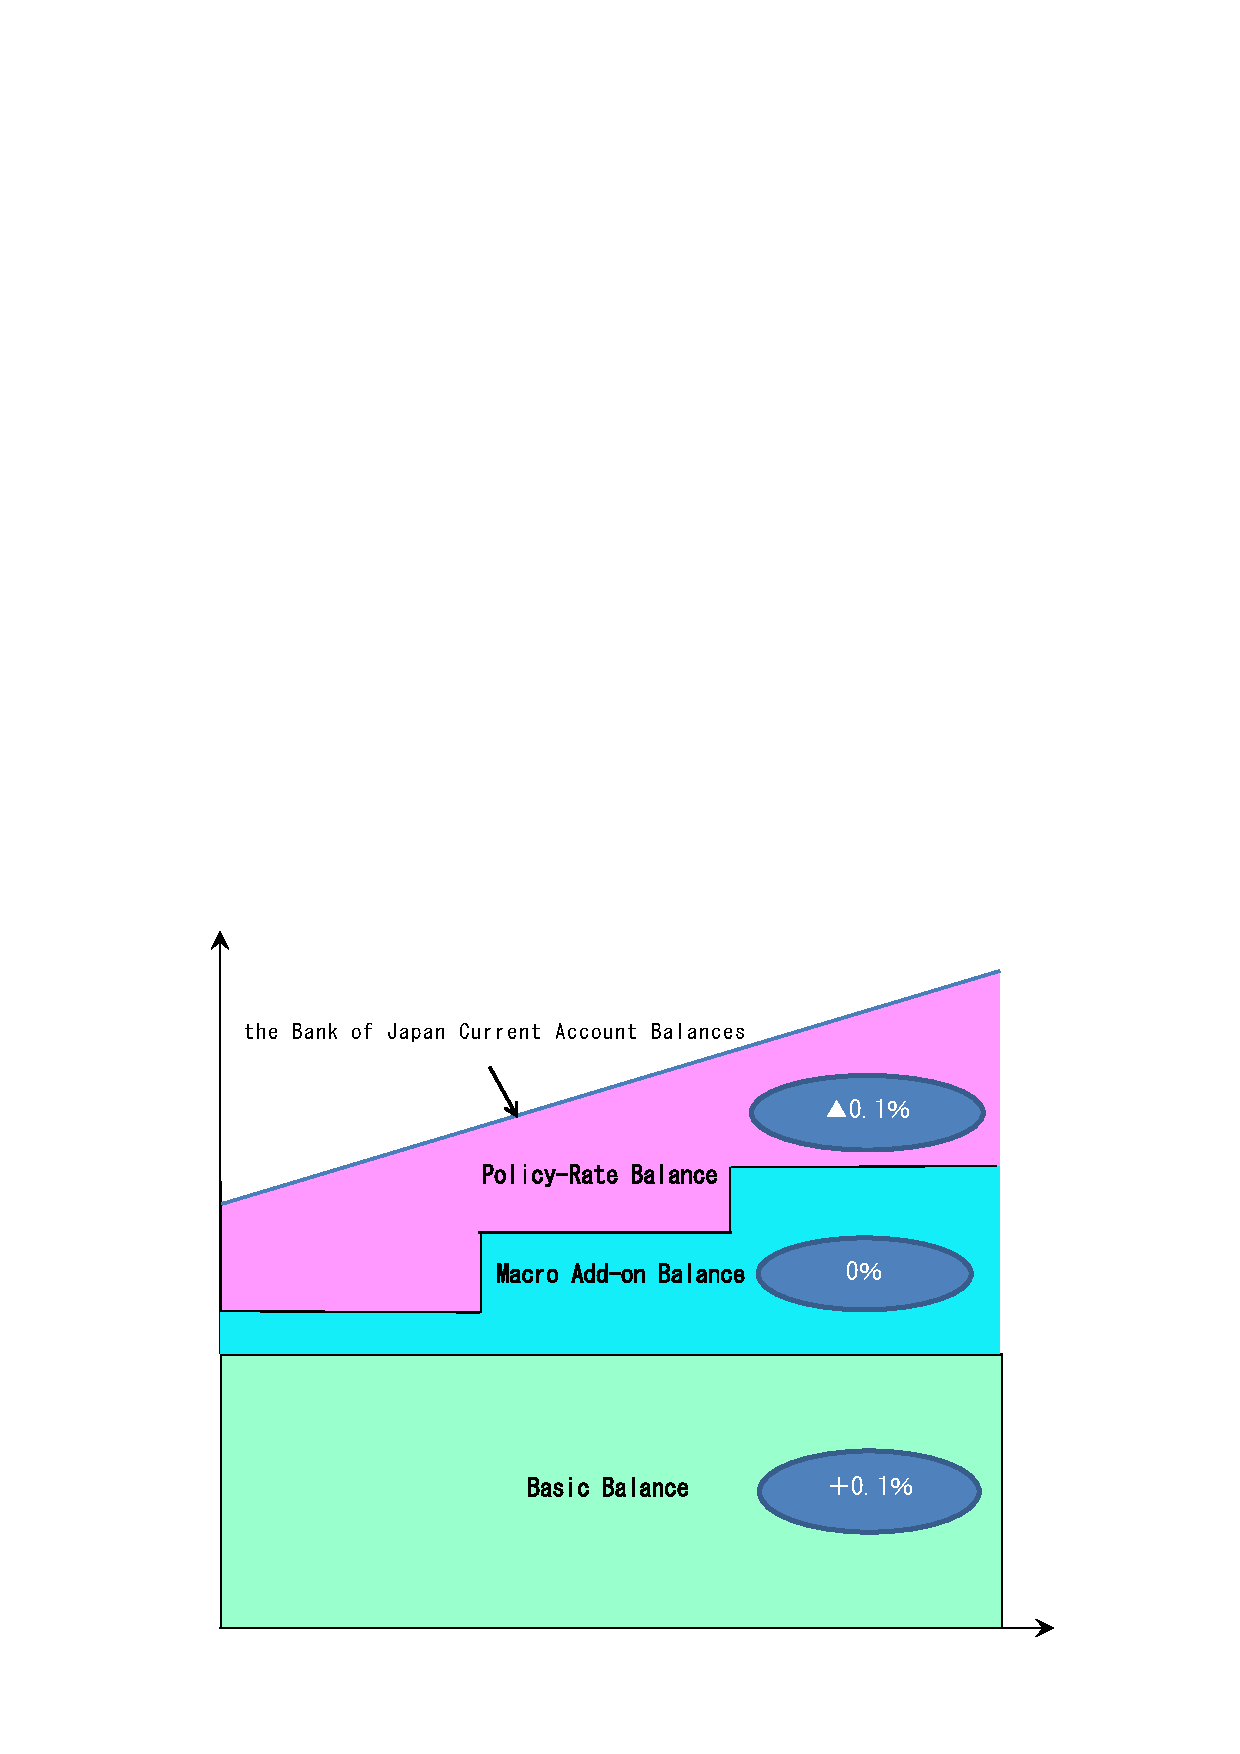
\includegraphics[width=17cm]{currentaccount.pdf}

  日本銀行 2016年1月29日「本日の決定のポイント」より引用
\end{figure}

%まず,ゼロ金利政策の効果の検証としては時間軸効果を中心に検討しているものが存在する。ゼロ金利政策下では時間軸効果は短期金利の将来経路に関する金融市場の期待を安定化させるためにきわめて重要であり,さらなる緩和効果を生み出すことができるとされた。しかし,白塚,藤木 (2001)及び翁,白塚 (2003)では瞬間フォワードレートカーブの分析をもとに金融部門と非金融部門の間の波及メカニズムが機能しない状況下では,金融部門の外部へ金融緩和の影響が波及しないことが示された。ゼロ金利政策期間においては金融政策単独では,金融市場における低成長とデフレが持続するという期待を反転させるには至らなかったと結論付けられている。

%また,Honda et al. (2013)及び原田,増島 (2010)では,変数間の相互関係が再帰的な関係であると仮定したCholesky分解を用いて分析されており,マネタリーベースの増加が生産を増加させる効果があることが示されたが,資産価値や銀行のバランスシートを通じる経路が主であり,時間軸効果を通じる経路は確認されなかった。量的緩和が長期的に金利を引き上げる効果も示され,時間軸効果の存在には疑問が持たれている。

%その他,原田・石橋 (2018)やHonda (2014),Kuttner (2018)では金融政策ショックが予想インフレ率などを波及経路として生産への明確なプラスの効果を与えたとされている。
%また,金融市場への影響についての研究としてはWright (2011),柴本 (2012)が挙げられる。Wright (2011)では政策アナウンス日,非アナウンスメント日における分散不均一性を仮定した構造型VARモデルを用いた分析により金融政策ショックが長期金利,短期金利,社債の利回りを下落させることが示された。
%また,同様の手法を用いた柴本 (2012)では日本の量的金融緩和ショックが短期的には長短金利差を低下させる一方,長期的には株価の上昇を伴いつつ,長短金利差も上昇させることが示された。

%他にも政策アナウンス日,非アナウンスメント日における分散不均一を仮定した構造型ベクトル自己回帰モデル (以下,構造型VARモデル)を用いて金融政策ショックを識別した先行研究もある。構造型VARモデルの特徴は指標としての金融政策ショックの識別と量的緩和政策発動直後の直接的な影響だけでなく,タイムラグを伴った影響を同時に分析できる点である。Wright (2011)では上記のモデルを用いて金融政策ショックが長期金利,短期金利,社債の利回りを下落させることが示された。しかし,効果の低減はかなり早く,半減期は約2ヶ月と推定された。また,柴本 (2012)では日本の量的金融緩和ショックが短期的には長短金利差を低下させる一方,長期的には株価の上昇を伴いつつ,長短金利差も上昇させることが示された。

\newpage
\subsection{欧州の金融緩和政策の影響,波及効果}

近年の欧州のデータで同様にCholesky分解を用いた構造型VARモデルを使用して,金融政策の物価への影響を分析した先行研究としてはPazicky [2018]が存在する。金融緩和政策の有効性については,
%金利が一定水準以下に低下した場合に金融政策が無効化される状況である,流動性の罠があるにもかかわらず,
長期金利の低下を主とした時間軸効果が働くことで長期的に経済に働くことが示唆されている。

その他,金融市場への影響を分析した先行研究としてはFratzscher et al. [2014]やEser and Schwaab [2016],Meszaros and Kiss [2020]などが挙げられる。
まず,Fratzscher et al. [2014]は欧州の金融政策の影響を初めて定量化した論文の1つであり,パネルデータやVARモデルを用い,資産価格への影響を分析したものである。
ここではSMPがユーロ圏の資産価格を増加させた一方で,ポートフォリオ・リバランス効果は見られなかったと結論付けられている。さらに,これが世界の株式市場に波及したことについても触れられている。
Eser and Schwaab [2016]ではユーロ圏の長期金利への影響が分析されており,SMP導入により対象国の国債のリスクプレミアムが減少し,短期的にも長期的にも長期金利を低下させる影響を持つと結論づけられた。また,アナウンスメントの効果としてはSMP開始の発表は大きな効果があったとされている。
Meszaros and Kiss [2020]ではリーマン・ショック以降のECBの金融緩和について,国債利回り,株価指数,為替レートに対する影響とその波及経路について分析が行われている。ここでは,ポートフォリオ・リバランス効果について,有価証券や外貨準備,貸付の増加などの変化があったとされており,これによって国債利回りの低下や為替レートの自国通貨安に効果が波及し,他の様々なチャネルを通して,株価の上昇に対しても影響があったと結論付けられている。

以上のように,欧州の金融政策の波及経路としては,ポートフォリオ・リバランス効果については肯定的な先行研究も懐疑的なものも両方存在するが,長期金利の低下については肯定的なものが多い。このように,中銀預金金利の利下げが複数回行なわれている欧州では市場の将来の短期金利についての予測が低下する,時間軸効果が働いているとしている先行研究が多い。

他にも,Demir [2014]では金融政策の為替レートへの影響について分析されているが,有意な影響は確認されたものの,量的な影響は小さいことが示唆されている。Haitsma et al. [2016]では株価指数,ユーロストックス50指数 (STOXX50)に対して正の影響を与え,特にバリュー株などにこの傾向がみられると結論付けられている。

\newpage

\section{分析手法}

\subsection{構造型VARモデル}

本稿の分析においては,第2章であげたHonda et al. [2013]及び原田・増島 [2009]で用いられているCholesky分解を用いた構造型VARモデルを使用した。
VARモデルは世界の中央銀行で広く使用されており,同時点間の影響をモデル化することが可能である。

Cholesky分解を用い,物価のほか,金融市場や外国為替市場への金融緩和政策の影響を分析した。
内生変数は後述する6変数を使用した。

本稿で分析の対象とする期間はリーマン・ショック以降の2009年から用いた変数全てのデータが得られた2019年末までである。この標本期間中,日本では2014年4月に消費増税の増税 (5\%→8\%)が行われている。
したがって,これの影響をモデルの推計の考慮に加えるため,日本のデータでの分析にのみ,消費増税のダミー変数を外生変数として加えた。

また,2019年10月にも消費税の増税 (8\%→10\%)が行われているが,軽減税率を導入し,食品(外食・酒類を除く)と宅配の新聞の定期購読料は現行の8\%の税率が維持されたことや,経済産業省により「キャッシュレス・ポイント還元事業」が行われたことから増税の影響は大きくないと判断し,こちらは考慮に加えない。

本稿の構造型VARモデルの推計については全ての変数に対し階差を取らず水準データを使用している。これについては本章第3節で述べる。

標準的なVARモデルでは,その分析から得られる結果から構造的錯乱項を識別することができないため,変数間の同時点の関係が考えられる場合,分析結果の政策的解釈が困難になる恐れがある。しかし,金利などの金融変数は金融ショックに対して1日以内の素早い反応を示すことが予想されるため,本稿では変数間の同時点間の関係性を考慮することのできるCholesky分解を用いた構造型VARモデルを採用する。
Cholesky分解を用いた構造型VARモデルでは同時点間の関係性を考慮するために係数行列$A_0$をモデルに組み込む。ここでは以下のような短期制約を課したモデルを想定する。

\begin{equation}
  \label{eq1}
  A_{0} y_{t} = \alpha + \sum_{k=1}^{n} B_{k} y_{t-k} + \varepsilon_t
\end{equation}

$y_t$は内生変数を表す$m$次元のベクトル,$n$は内生変数のラグ,$\varepsilon$は$m$次元の構造ショックを表すベクトル,$\alpha$は定数項,$A_0$,$B_0$から$B_k$は$m \times m$の正方行列である。上記の構造型VARモデルは直接推計できないため,$A_0$の逆行列を両辺に乗じる。

\begin{equation}
  \label{eq2}
  y_t =A_0^{-1} \alpha + \sum_{k=1}^{n} C_{k} y_{t-k} +e_t
\end{equation}

$C_k$は$(A_0^{-1})\times B_k$である。また$e_{t}$は $A_0^{-1} \varepsilon_t$である。

原田・増島 [2009]では$A_0^{-1}$が式(\ref{eq3})のような下三角行列であるという制約を課している。この条件では$y_t$の$s$行目$(0 < s \leq m)$の内生変数は1行目から$s$行目までの内生変数における構造ショックの影響は受けるが,$s + 1$行目以降の内生変数における構造ショックの影響は受けない。この制約下においては変数の順序により結果が異なるため,外生性の高い変数がベクトルの上にくるように配列する必要がある。本稿では後述する金融政策変数が物価上昇にどのような影響を与えるのかを分析するため,金融政策変数,株価などの金融変数,物価指数の順序で並べ分析を行った。

\begin{equation}
  \label{eq3}
  A_0^{-1} = \left[
    \begin{array} {cccc}
      x      & 0      & \ldots & 0      \\
      \vdots & \ddots & \ddots & \vdots \\
      \vdots & \      & \ddots & 0      \\
      x      & \ldots & \ldots & x
    \end{array}
    \right]
\end{equation}

また,このVARモデルにおけるラグは日本を1,欧州を2とする。これは赤池情報量基準 (AIC)により選択されている。

\subsection{ダミー変数と重回帰式}

本稿では上記の構造型VARでの分析に加え,日本銀行によるアナウンスメントが物価に対しどのような効果を与えたかについて分析するため,ダミー変数を用いた重回帰分析を行った。

構造型VARモデルでは政策ダミー変数を外生変数としてモデルに組み込むことはできるが,それでは物価目標へのコミットメントを行うアナウンスメントの効果を測ることが困難である。
そのため,本稿では政策ダミー変数を説明変数に加えた重回帰分析を行うことでこの効果を測定する。
この政策ダミー変数は物価目標へのコミットメントを行うアナウンスメントが物価に与える影響を見るために政策開始日よりも前は0,以後1をとる変数である。これによって中央銀行の方針の転換によって引き起こされた変化を考慮することが可能になる。
前述のとおり,ECBは2003年より物価目標の変更を行っておらず,金融緩和政策期間中での物価への影響を分析できないため,この分析は行わなかった。

したがって,物価指数を目的変数とし,政策変数であるマネタリーベースを除いた,その他の構造型VARで用いたものと同様の金融変数に加え,政策ダミー変数を説明変数とした以下の重回帰式を使用した。
なお,前述の構造型VARモデルと同様に消費増税の影響を考慮に入れるため,説明変数に消費増税ダミー変数を加えており,説明変数の数は6である。

\begin{equation}
  \label{eq4}
  \begin{gathered}
    y_i = \beta_0 + \sum_{j=1}^k \beta_j X_{ij} + \varepsilon_i \\
    i=1,2,...n :観測値のインデックス\\
    j=1,2,...k :説明変数の数\\
    %y_i: 消費者物価指数   X_1: 短期金利 X_2: 長期金利\\
    %X_3: 為替レート X_4: 株価指数 X_5: 政策ダミー変数 X_6: 消費増税ダミー変数
  \end{gathered}
\end{equation}

ここで$y_i$は従属変数,$\beta_0$はモデルの切片,$X_ij$はモデルの$j$番目の説明変数 ($j$= 1からk),$\varepsilon_i$は期待値0,分散$\sigma^2$である確率誤差モデルの誤差項である。

これを行列式で表すと次の式である。

\begin{equation}
  \label{eq5}
  \left[
    \begin{array} {c}
      y_1    \\
      y_2    \\
      \vdots \\
      y_n    \\
    \end{array}
    \right]
  =
  \left[
    \begin{array} {c}
      1,x_{11},x_{21},\cdots x_{k1}                                         \\
      1,x_{12},x_{22},\cdots x_{k2}                                         \\
      \vdots \hspace{20pt} \vdots \hspace{20pt} \vdots \hspace{20pt} \vdots \\
      1,x_{1n},x_{2n},\cdots x_{kn}                                         \\
    \end{array}
    \right]
  \cdot
  \left[
    \begin{array} {c}
      \beta_0 \\
      \beta_1 \\
      \beta_2 \\
      \vdots  \\
      \beta_k \\
    \end{array}
    \right]
  +
  \left[
    \begin{array} {c}
      \varepsilon_1 \\
      \varepsilon_2 \\
      \vdots        \\
      \varepsilon_n \\
    \end{array}
    \right]
\end{equation}

これを簡単化すると,次の式を得る。

\begin{equation}
  \label{eq6}
  Y = X B + E
\end{equation}

これを用いて,$B$の推定量を計算する。

\begin{equation}
  \label{eq7}
  \hat{B}=(X^T \cdot X)^{-1} \cdot X^T \cdot Y
\end{equation}

%n個のオブザベーションがある場合,i番目のオブザベーションでの従属変数の予測値は次式で計算できる。

%\begin{equation}
%\label{eq5}
%y_i = \beta_0 + \sum_{j=1}^n \beta_j X_{ij}
%\end{equation}

%観察値と予測値の間の2乗距離の合計を最小化することで以下のモデルのパラメータの推定を行う。

%\begin{equation}
%\label{eq6}
%\beta = (X'DX)^{-1}X'Dy \sigma^2 = \frac{1}{W-p^*} \sum_{j=1}^n w_i(\bar{y_i} y_i)
%\end{equation}

%ここで$\beta$は$\beta_i$パラメータの推定値のベクトル,$X$は1のベクトルで始まる説明変数の行列, $y$は従属変数のn個の観察値のベクトル,$w_i$ はi 番目のオブザベーションの重みで,W は$w_i$の重みの合計,Dは対角線上に$w_i$の重みを持つ行列である。

\newpage

\subsection{分析の問題点}

Cholesky分解を用いた構造型VARモデルでは変数の順序が重要であり,順序が変われば異なる結果になることが知られている。これは変数の順序が早いほど,その変数のショックがほかの変数に与える影響が大きいためである。そのため,変数の外生性については十分に吟味される必要がある。本稿の分析においてはいくつかの順序を変えた変数のセットでの分析を行い,適切な順序の特定を試みた。本稿では最も適当と考えられる変数の順序の分析結果を掲載している。

今回の構造型VARモデルの推計については全ての変数に対し階差を取らず水準データを使用した理由としては,誘導型VARモデルの推計に関して非定常な変数が含まれていても,構造型VARモデルの推計における推定量は一致性を持つことが知られているためである。
照山 [2001]では VARモデル を用いた金融政策の分析についての展望論文において,たとえ水準タームで非定常系列を含む場合でも,そのままで推計する方法が中心となっていることが紹介されている。これは,Sims et al. [1990]による,非定常な変数が含まれている場合にも,水準による推定量が一致性を持つことに依存している。
なお,非定常な変数が含まれる場合,インパルス応答関数の信頼区間は必ずしも適切ではないが,本稿では参考のため掲載している。

また,金融緩和政策の波及経路としては予想物価上昇率や実質金利に注目している先行研究も多い。実質金利は名目金利から予想物価上昇率を引くことで求められるが,国際通貨基金 (IMF)が公開している予想物価上昇率のデータは年次データであるため,本稿の分析では使用が難しい。この問題に対処するため,本稿では予想物価上昇率や実質金利の影響を受けると考えられる株価と為替レートを代替の金融変数として用いた。

以上の分析手法のもと,金融政策と物価上昇との関係を分析し,頑健性を得るとともに,波及経路の特定を試みた。

\newpage

\section{データ}

構造型VARモデルのデータとしては標本期間を2009年1月から2019年12月までの月次データを採用している。これはリーマン・ショック以後の日本と欧州に,金融政策がどのような影響を与えたかを分析するためである。また,データが月次となっているのはECBが各マクロデータを月ごとの公開としているためである。対して,日本銀行は毎日のデータ公開を行っているが,欧州のデータとサンプル数を合わせるため,日本のデータも月次で用いた。
変数はそれぞれ,$JMB$,$JSTOCK$,$JLIBOR$,$JBOND$,$USDJPY$,$JCPI$と$EMB$,$ESTOCK$,$ELIBOR$,$EBOND$,$USDEUR$,$EHICP$の6つずつ用いた。
また,日本のデータでのVAR分析にのみ外生変数として用いた消費増税ダミー ($TAXDUMMY$)は2014年4月より前を0,以後を1とするダミー変数である。

量的・質的金融緩和の指標としてマネタリーベース(ベースマネー)を金融政策変数 ($JMB,EMB$)として用いた。他に政策変数の候補としてはマネーストックや日銀当座預金残高も検討したが,マネーストックに対する金融緩和の影響は限定的であるため,金融政策変数として適切ではない。また,日銀当座預金残高についても物価上昇に対する流通現金の影響は小さくないと考えられるため,日銀当座預金残高に流通現金を加えたものであるマネタリーベースを採用した。
残りの金融市場の変数としては$JSTOCK,ESTOCK$に株式市場の指標として日経平均株価指数 (Nikkei255)とユーロストックス50指数(STOXX50)を用いた。また,金利については比較を容易にするため,$JLIBOR,ELIBOR$に短期金利の指標としてそれぞれロンドン銀行間取引金利 (LIBOR)の円ベース3ヶ月金利とユーロベース3ヶ月金利を,$JBOND,EBOND$に長期金利の指標として各国政府が公表している日本国債10年物利回りとドイツ上場連邦証券10年物利回りを用いた。その他,為替レートは輸入物価を通して物価上昇への影響があると考えられるため変数として加えている。$USDJPY$に外国為替市場の指標として日本銀行が公開している東京市場のドル・円スポットレートを,$USDEUR$にECBが発表しているドル・ユーロ間の外国為替基準レートを用いた。日本と欧州のデータの両方でドル基準のレートを使用したのは,アメリカのFRBは現在もなお,マイナス金利を導入していない状態であるほか,日本銀行とECBの両者と比べて金融緩和政策の効果が低いと考えられるためである。値はすべて終値を用いている。

政策の効果を測るための物価変動の指標 ($JCPI$)としては生鮮食品とエネルギーを除いた消費者物価指数 (コアコアCPI)を用いた。生鮮食品・エネルギーを除いた指標を用いているのは生鮮食品の価格の変動が大きく,エネルギーは原油価格の大幅下落があったため,物価の基調が捉えられないためである。コアコアCPIのデータとしては総務省が公開している月次データを用いた。
%日次データが公開されている東大日次物価指数や一橋指数を用いなかった理由としてはこれらが主に日用品の販売データから算出された指数であるのに対し,総務省が公開しているCPIではより幅広い品目を対象としているためである。

また,欧州ではこれと類似する物価変動の指標 ($EHICP$)として食品とエネルギーを除いたEU基準消費者物価指数を用いた。これはEU加盟国でのマーストリヒト条約統一基準に基づく物価指数であり,ECBが公表する欧州の物価指数として最もコアコアCPIに類似したものだと考えられるためである。

$JCPI$,$EHICP$ともに2015年を基準とし、2015年の1年間のデータの平均を100とする指数に換算したものである。

これらのデータの詳細および出典は以下の表の通りである。なお,$JMB$,$EMB$,$JSTOCK$,$ESTOCK$,$USDJPY$,$JCPI$,$EHICP$は自然対数をとっている。

%金融政策ショックの識別では$MB, $$STOCK, $$BOND, $$C2CPI$の4変数を用いた。変数を落とした理由としては6変数では$R_1$を推定する最短距離問題を解けなかったためである。Cholesky分解においてCPIへの影響が小さいと考えられた$LIBOR,$ $USDJPY$を除いた。
%また,金融政策ショックの識別のためには政策日と非政策日の2つのサブサンプルに関して金融政策ショック以外の構造ショックの分散が一定である必要がある。そのため,本稿ではRigobon and Sack (2004)に従い,政策日を政策決定会合後に政策決定に関するアナウンスメントがあった日とし,非政策日を政策日の前取引日とした。本稿の標本期間中に57回の政策決定会合が実施されており,$R_1$を推定するためのサンプル数は114である。

重回帰分析におけるデータも政策変数 ($JMB$)を除いた同じデータセット ($JSTOCK$,$JLIBOR$,$JBOND$,$USDJPY$,$TAXDUMMY$)を用いた。これに加え,物価安定目標2\%のインフレターゲットが導入された2013年1月より前を0,以後1とする政策ダミー変数 ($ITDUMMY$)と,CPIの前年比上昇が2%を一時的に上回ってもすぐに金融緩和政策をやめるのではなく,同実績値が安定的に2%を超えるまでマネタリーベースの拡大を継続することが約束された「オーバーシュート型コミットメント」が出された2016年9月より前を0,以後1とする政策ダミー変数 ($OSDUMMY$)の2つの政策ダミー変数を用いた。

%%変数のリスト
\newpage
\begin{table}[H]
  \centering
  \caption{本稿の分析で用いた日本の変数}
  \vspace{10pt}
  \begin{threeparttable}
    \begin{tabular}{ccc} \toprule[0.5pt]\toprule[0.5pt]
      変数名     & 定義                                                     & 出典     \\ \midrule[0.5pt]
      $JMB$      & マネタリーベース (億円)                                  & 日本銀行 \\
      $JSTOCK$   & 日経平均株価指数 (Nikkei225)                             & 日経     \\
      $JLIBOR$   & ロンドン銀行間取引金利 (LIBOR・3ヶ月) (円ベース) (\%)    & FRED     \\
      $JBOND$    & 日本国債10年物利回り (\%)                                & 財務省   \\
      $USDJPY$   & 東京市場ドル・円 スポットレート (円/\$)                  & 日本銀行 \\
      $JCPI$     & 生鮮食品とエネルギーを除いた消費者物価指数 (コアコアCPI) & 総務省   \\
      $TAXDUMMY$ & 2014年4月より前を0,以降を1とする消費増税ダミー変数      &          \\
      $ITDUMMY$  & 2013年1月より前を0,以降を1とする政策ダミー変数          &          \\
      $OSDUMMY$  & 2016年9月より前を0,以降を1とする政策ダミー変数          &          \\
      \bottomrule[0.5pt]\bottomrule[0.5pt]
    \end{tabular}
    \vspace{10pt}
    \begin{tablenotes}\footnotesize
      \item[1]データはすべて月次データとした。
      \item[2] 時系列データはすべて終値を使用した。
      \item[3] $JMB,JSTOCK,USDJPY,JCPI$は自然対数をとっている。
    \end{tablenotes}
  \end{threeparttable}
\end{table}

\vspace{80pt}

\begin{table}[H]
  \centering
  \caption{本稿の分析で用いた欧州の変数}
  \vspace{10pt}
  \begin{threeparttable}
    \begin{tabular}{ccc} \toprule[0.5pt]\toprule[0.5pt]
      変数名   & 定義                                                      & 出典           \\ \midrule[0.5pt]
      $EMB$    & ECBベースマネー (100万ユーロ)                             & ECB            \\
      $ESTOCK$ & ユーロ・ストックス50指数 (STOXX50)                        & ECB            \\
      $ELIBOR$ & ロンドン銀行間取引金利 (LIBOR・3ヶ月) (ユーロベース) (\%) & FRED           \\
      $EBOND$  & ドイツ 上場連邦証券10年物利回り (\%)                      & ドイツ連邦銀行 \\
      $USDEUR$ & ECB参照為替レート (\euro /\$)                             & ECB            \\
      $EHICP$  & 食品とエネルギーを除いたEU基準消費者物価指数 (HICPexFE)   & ECB            \\
      \bottomrule[0.5pt]\bottomrule[0.5pt]
    \end{tabular}
    \vspace{10pt}
    \begin{tablenotes}\footnotesize
      \item[1] データはすべて月次データとした。
      \item[2] 時系列データはすべて終値を使用した。
      \item[3] $EMB$は一部の欠落したデータを3次補間法によりデータを内挿して用いている。
      \item[4] $EHICP$は季節調整されたデータがなかったことから「X-12-ARIMA」による季節調整を行った。
      \item[5] $EMB,ESTOCK,EHICP$は自然対数をとっている。
    \end{tablenotes}
  \end{threeparttable}
\end{table}

%%変数の推移
\begin{figure}[!htbp]
  \centering
  \caption{それぞれの変数の推移}
  \vspace{10pt}
  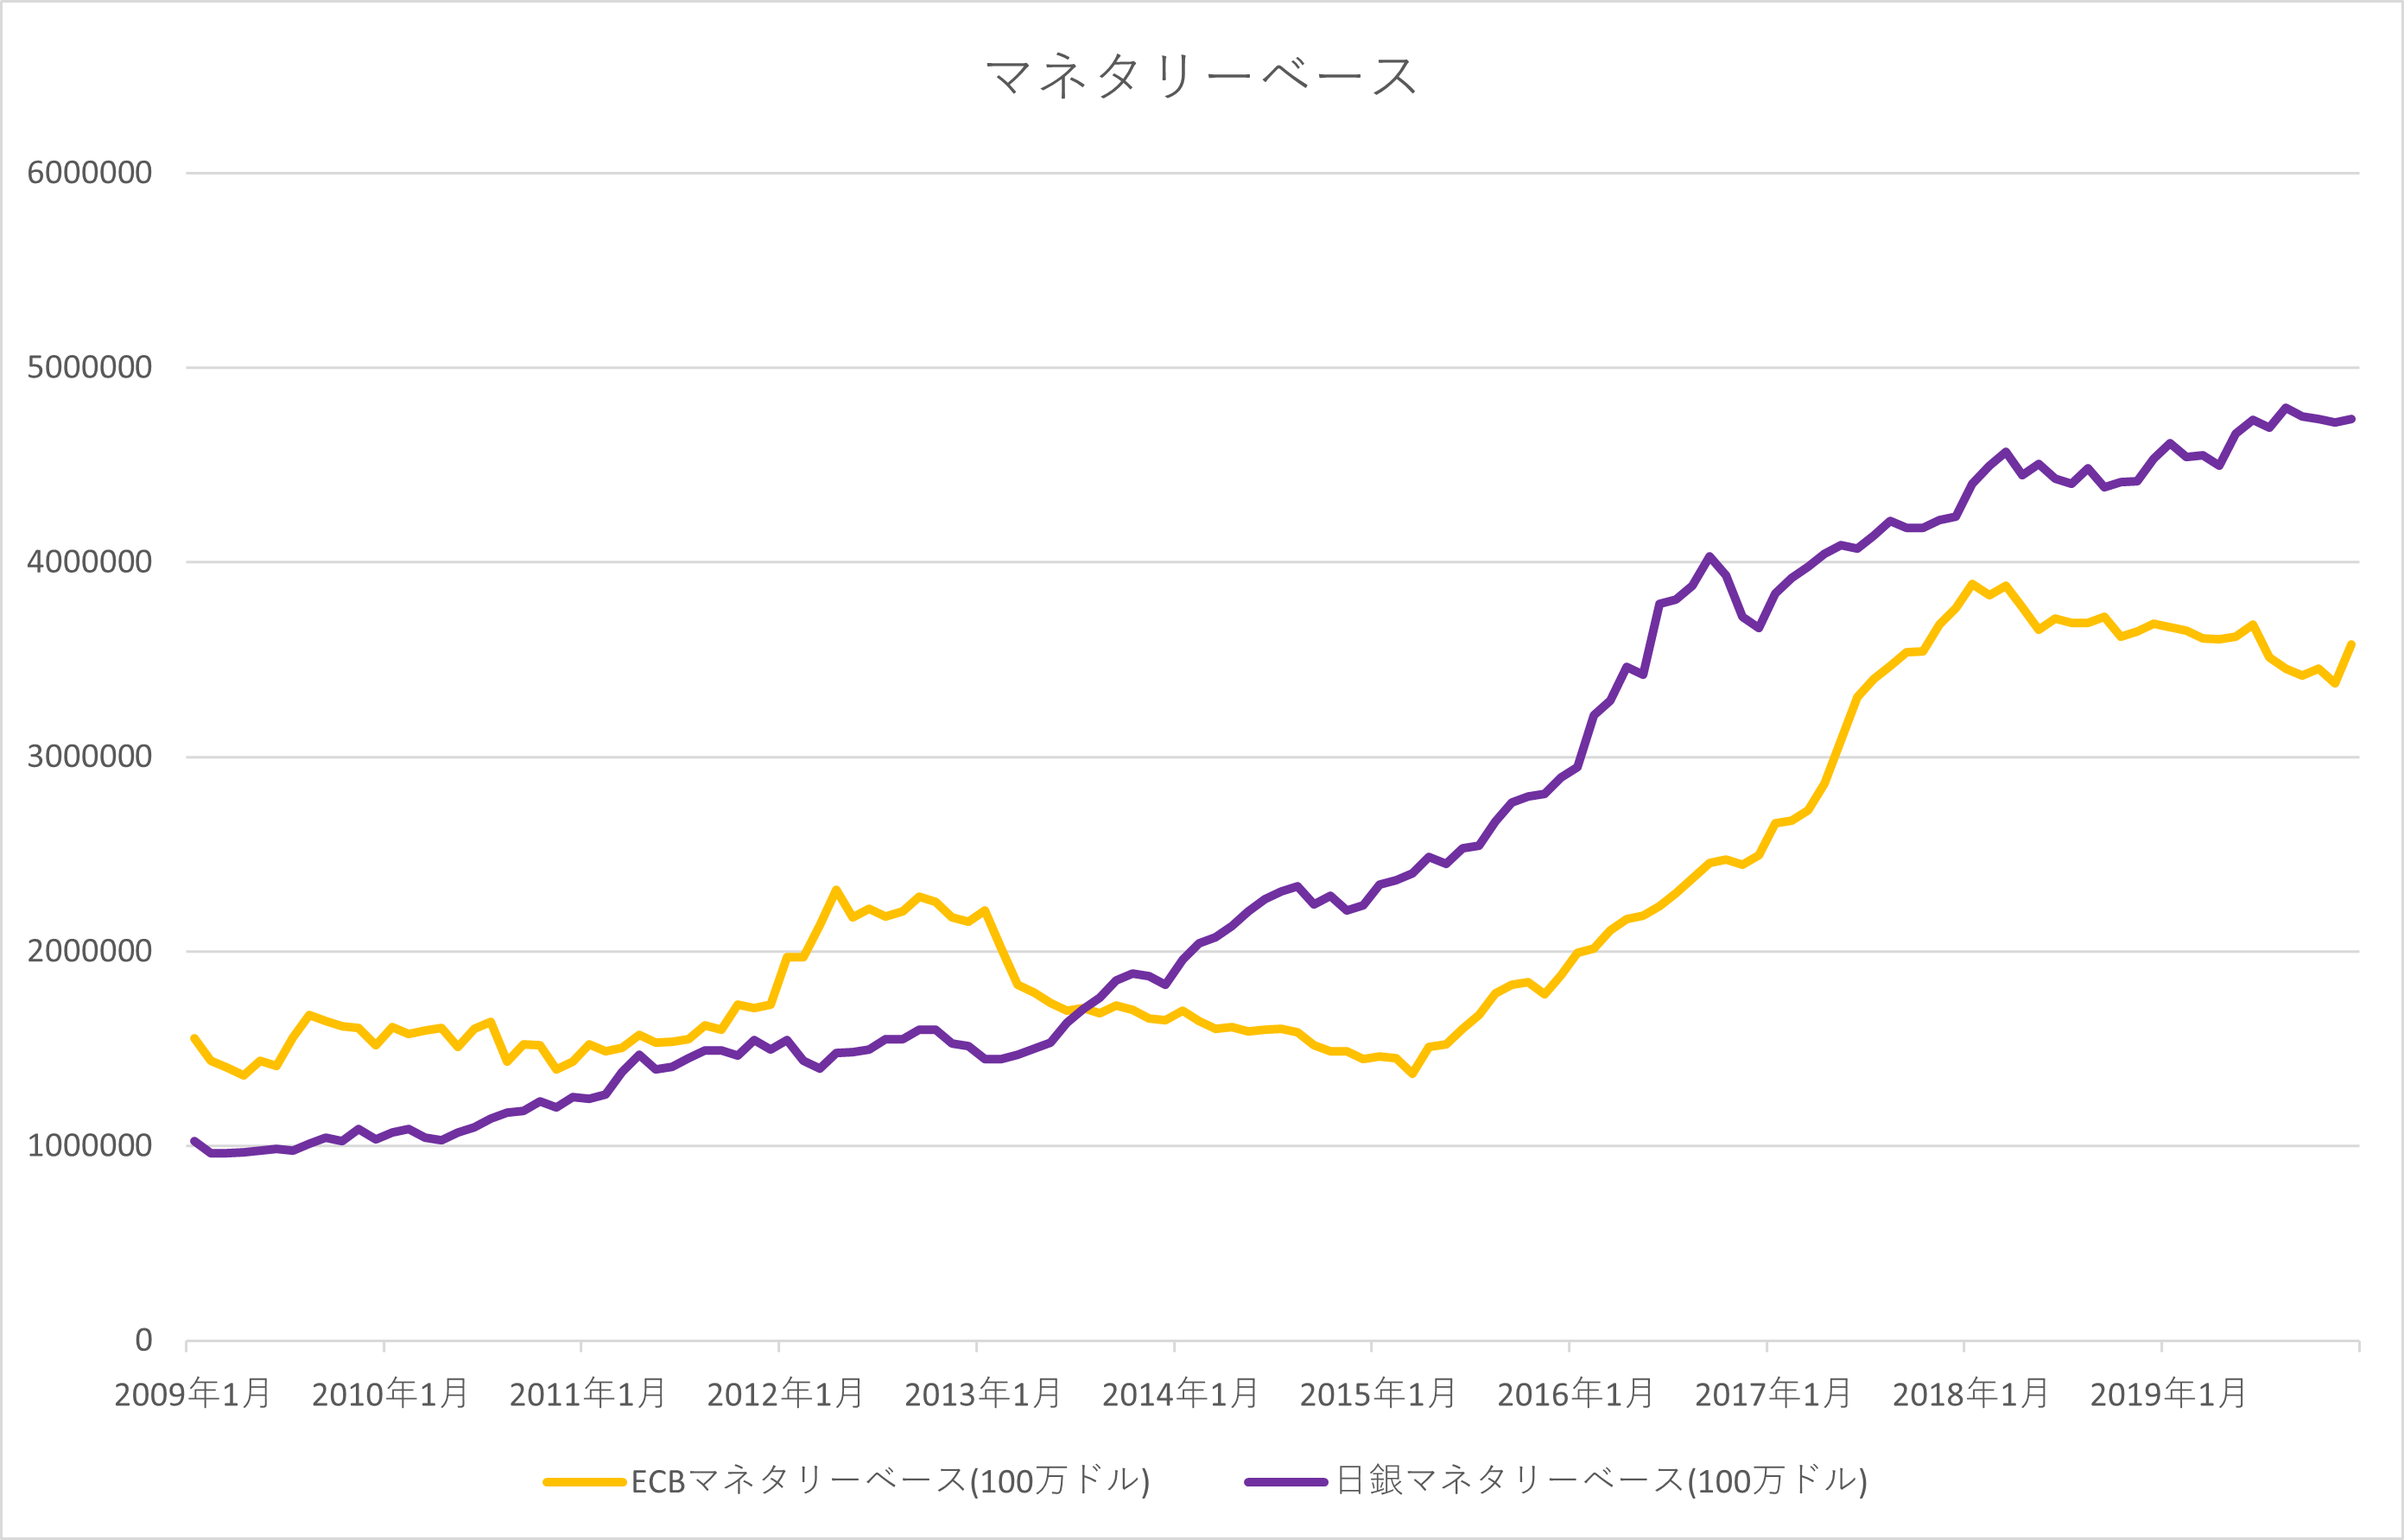
\includegraphics[width=16cm]{mbfix.png}
  \vspace{10pt}
  \begin{tablenotes}\footnotesize
    \item[1] $JMB$と$EMB$についてそれぞれ$USDJPY$,$USDEUR$を用いて単位を揃えた。
  \end{tablenotes}
  \vspace{10pt}
  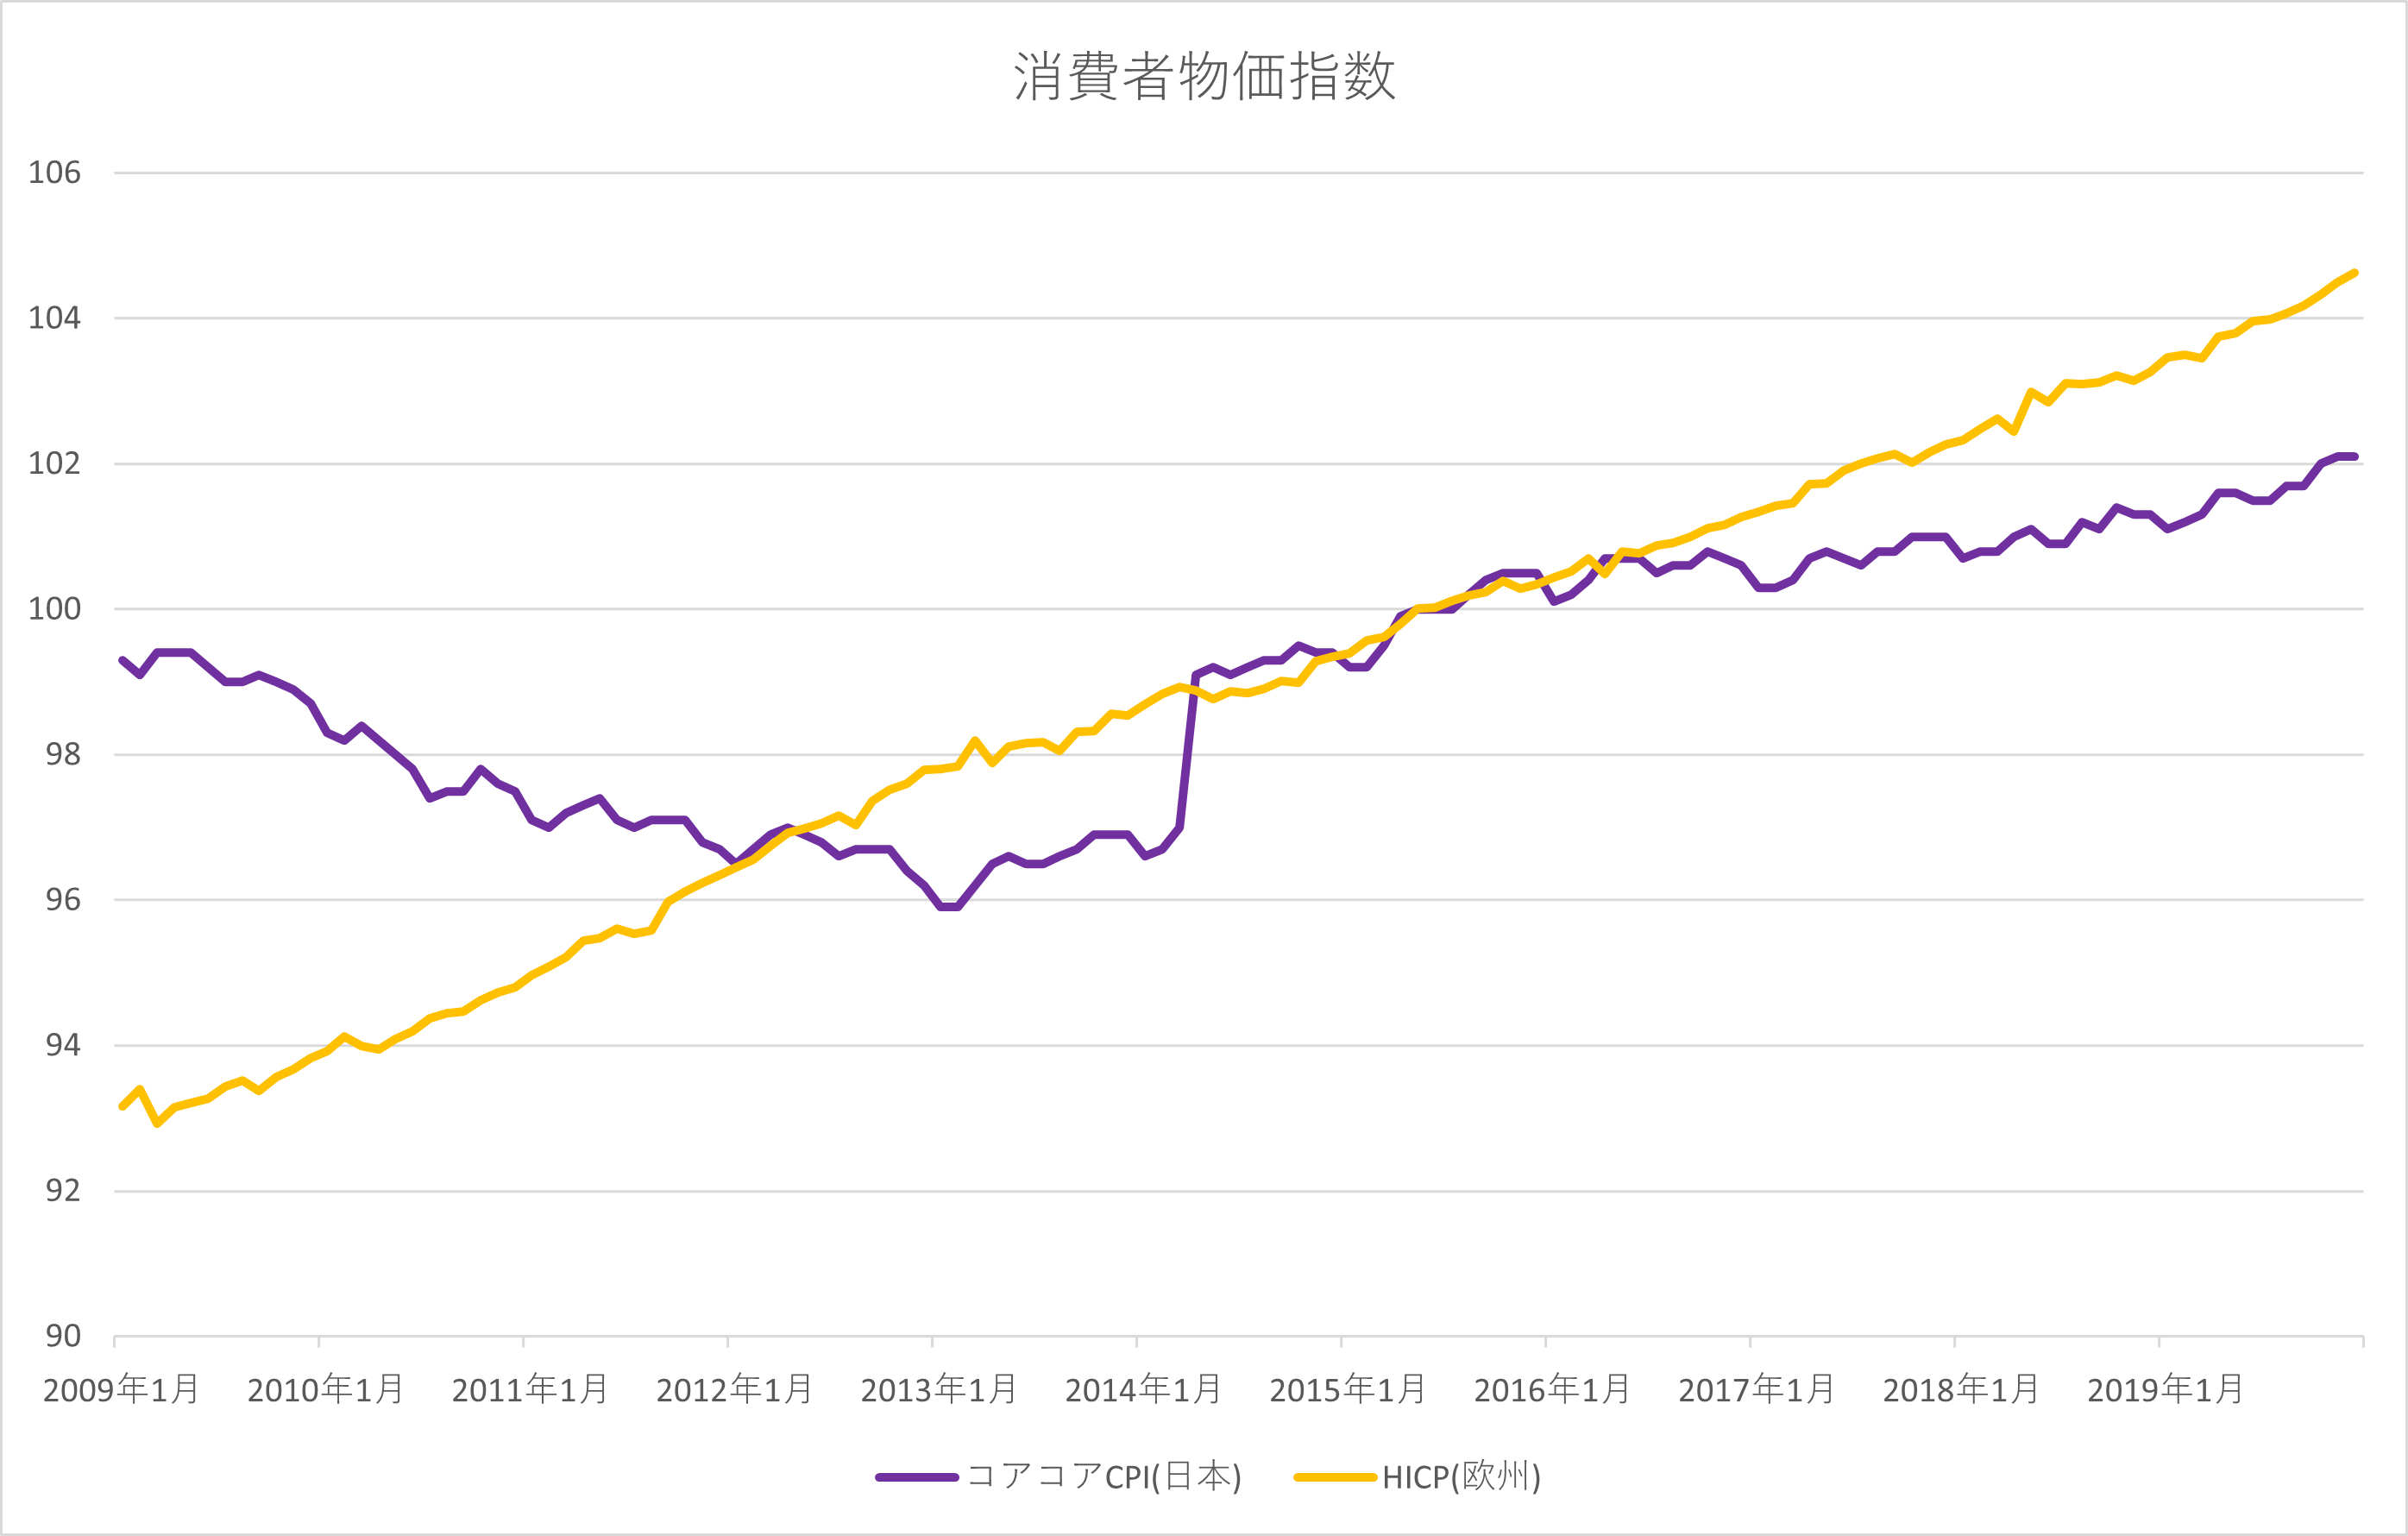
\includegraphics[width=16cm]{cpi09.png}
  \vspace{10pt}
  \begin{tablenotes}\footnotesize
    \item[1] $JCPI$,$EHICP$ともに2015年の1年間の平均を100とした指数である。
  \end{tablenotes}
\end{figure}

\newpage
\begin{figure}[!htbp]
  \centering
  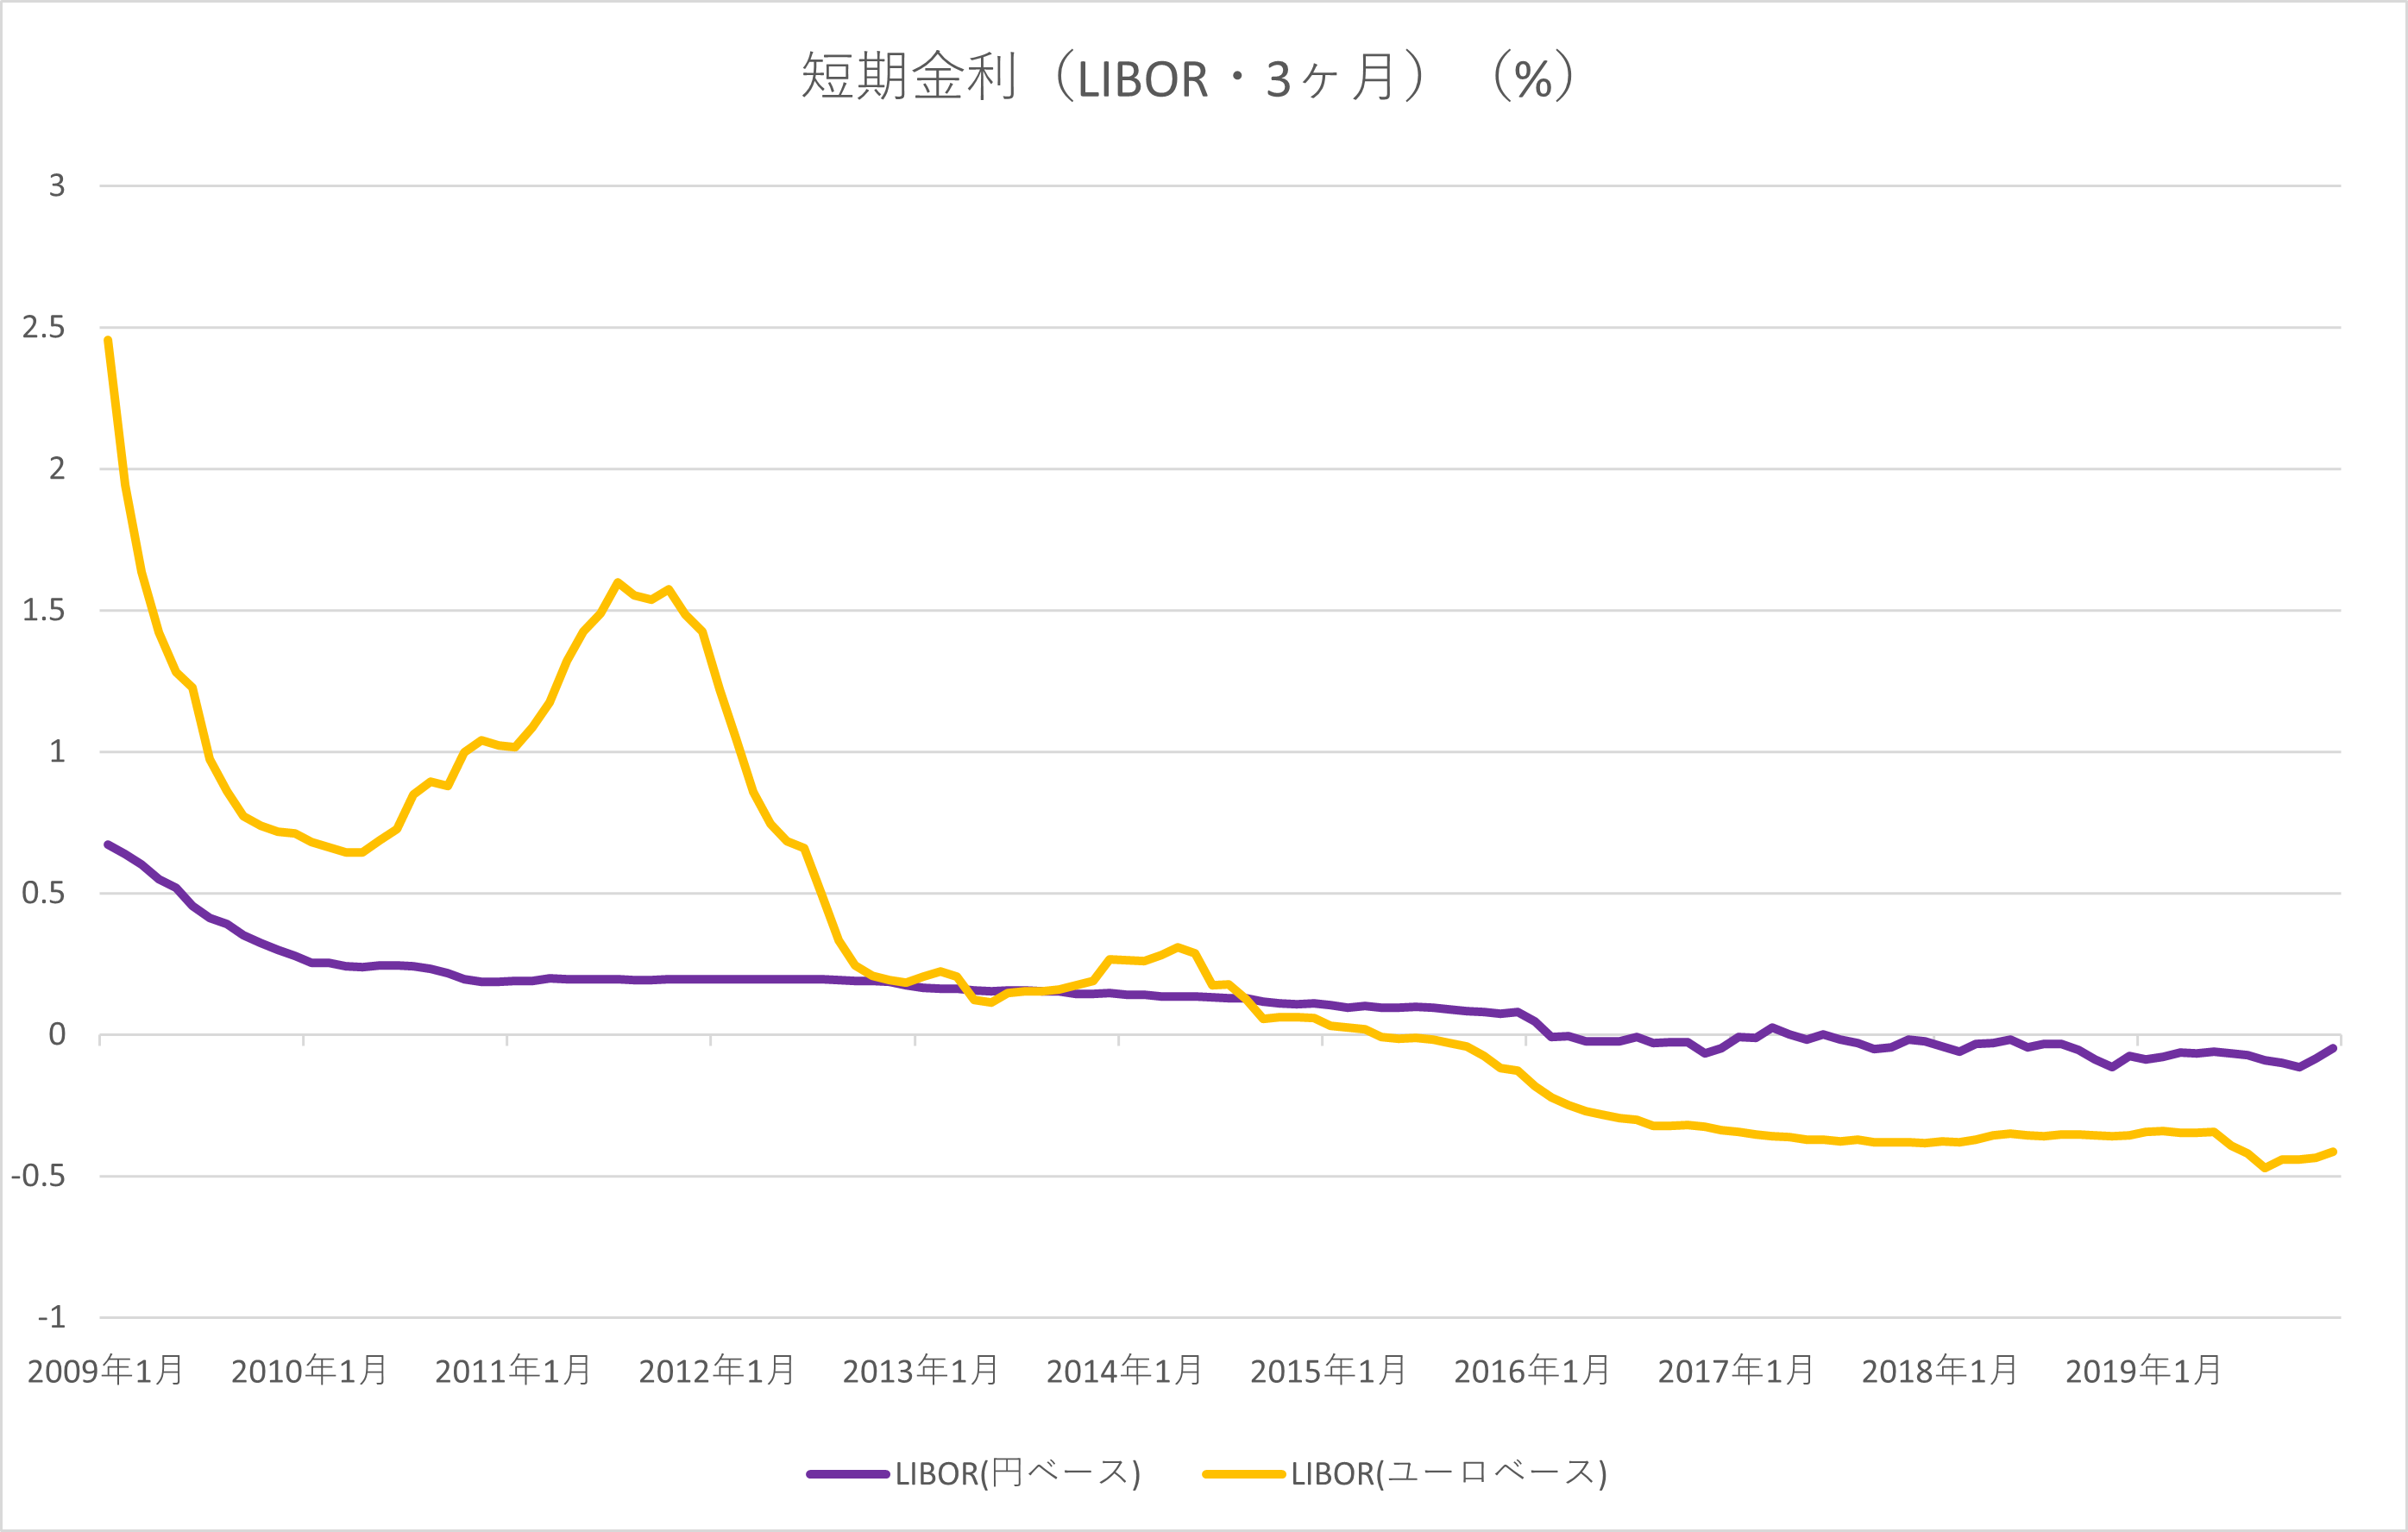
\includegraphics[width=16cm]{libor09.png}
\end{figure}
\begin{figure}[!htbp]
  \centering
  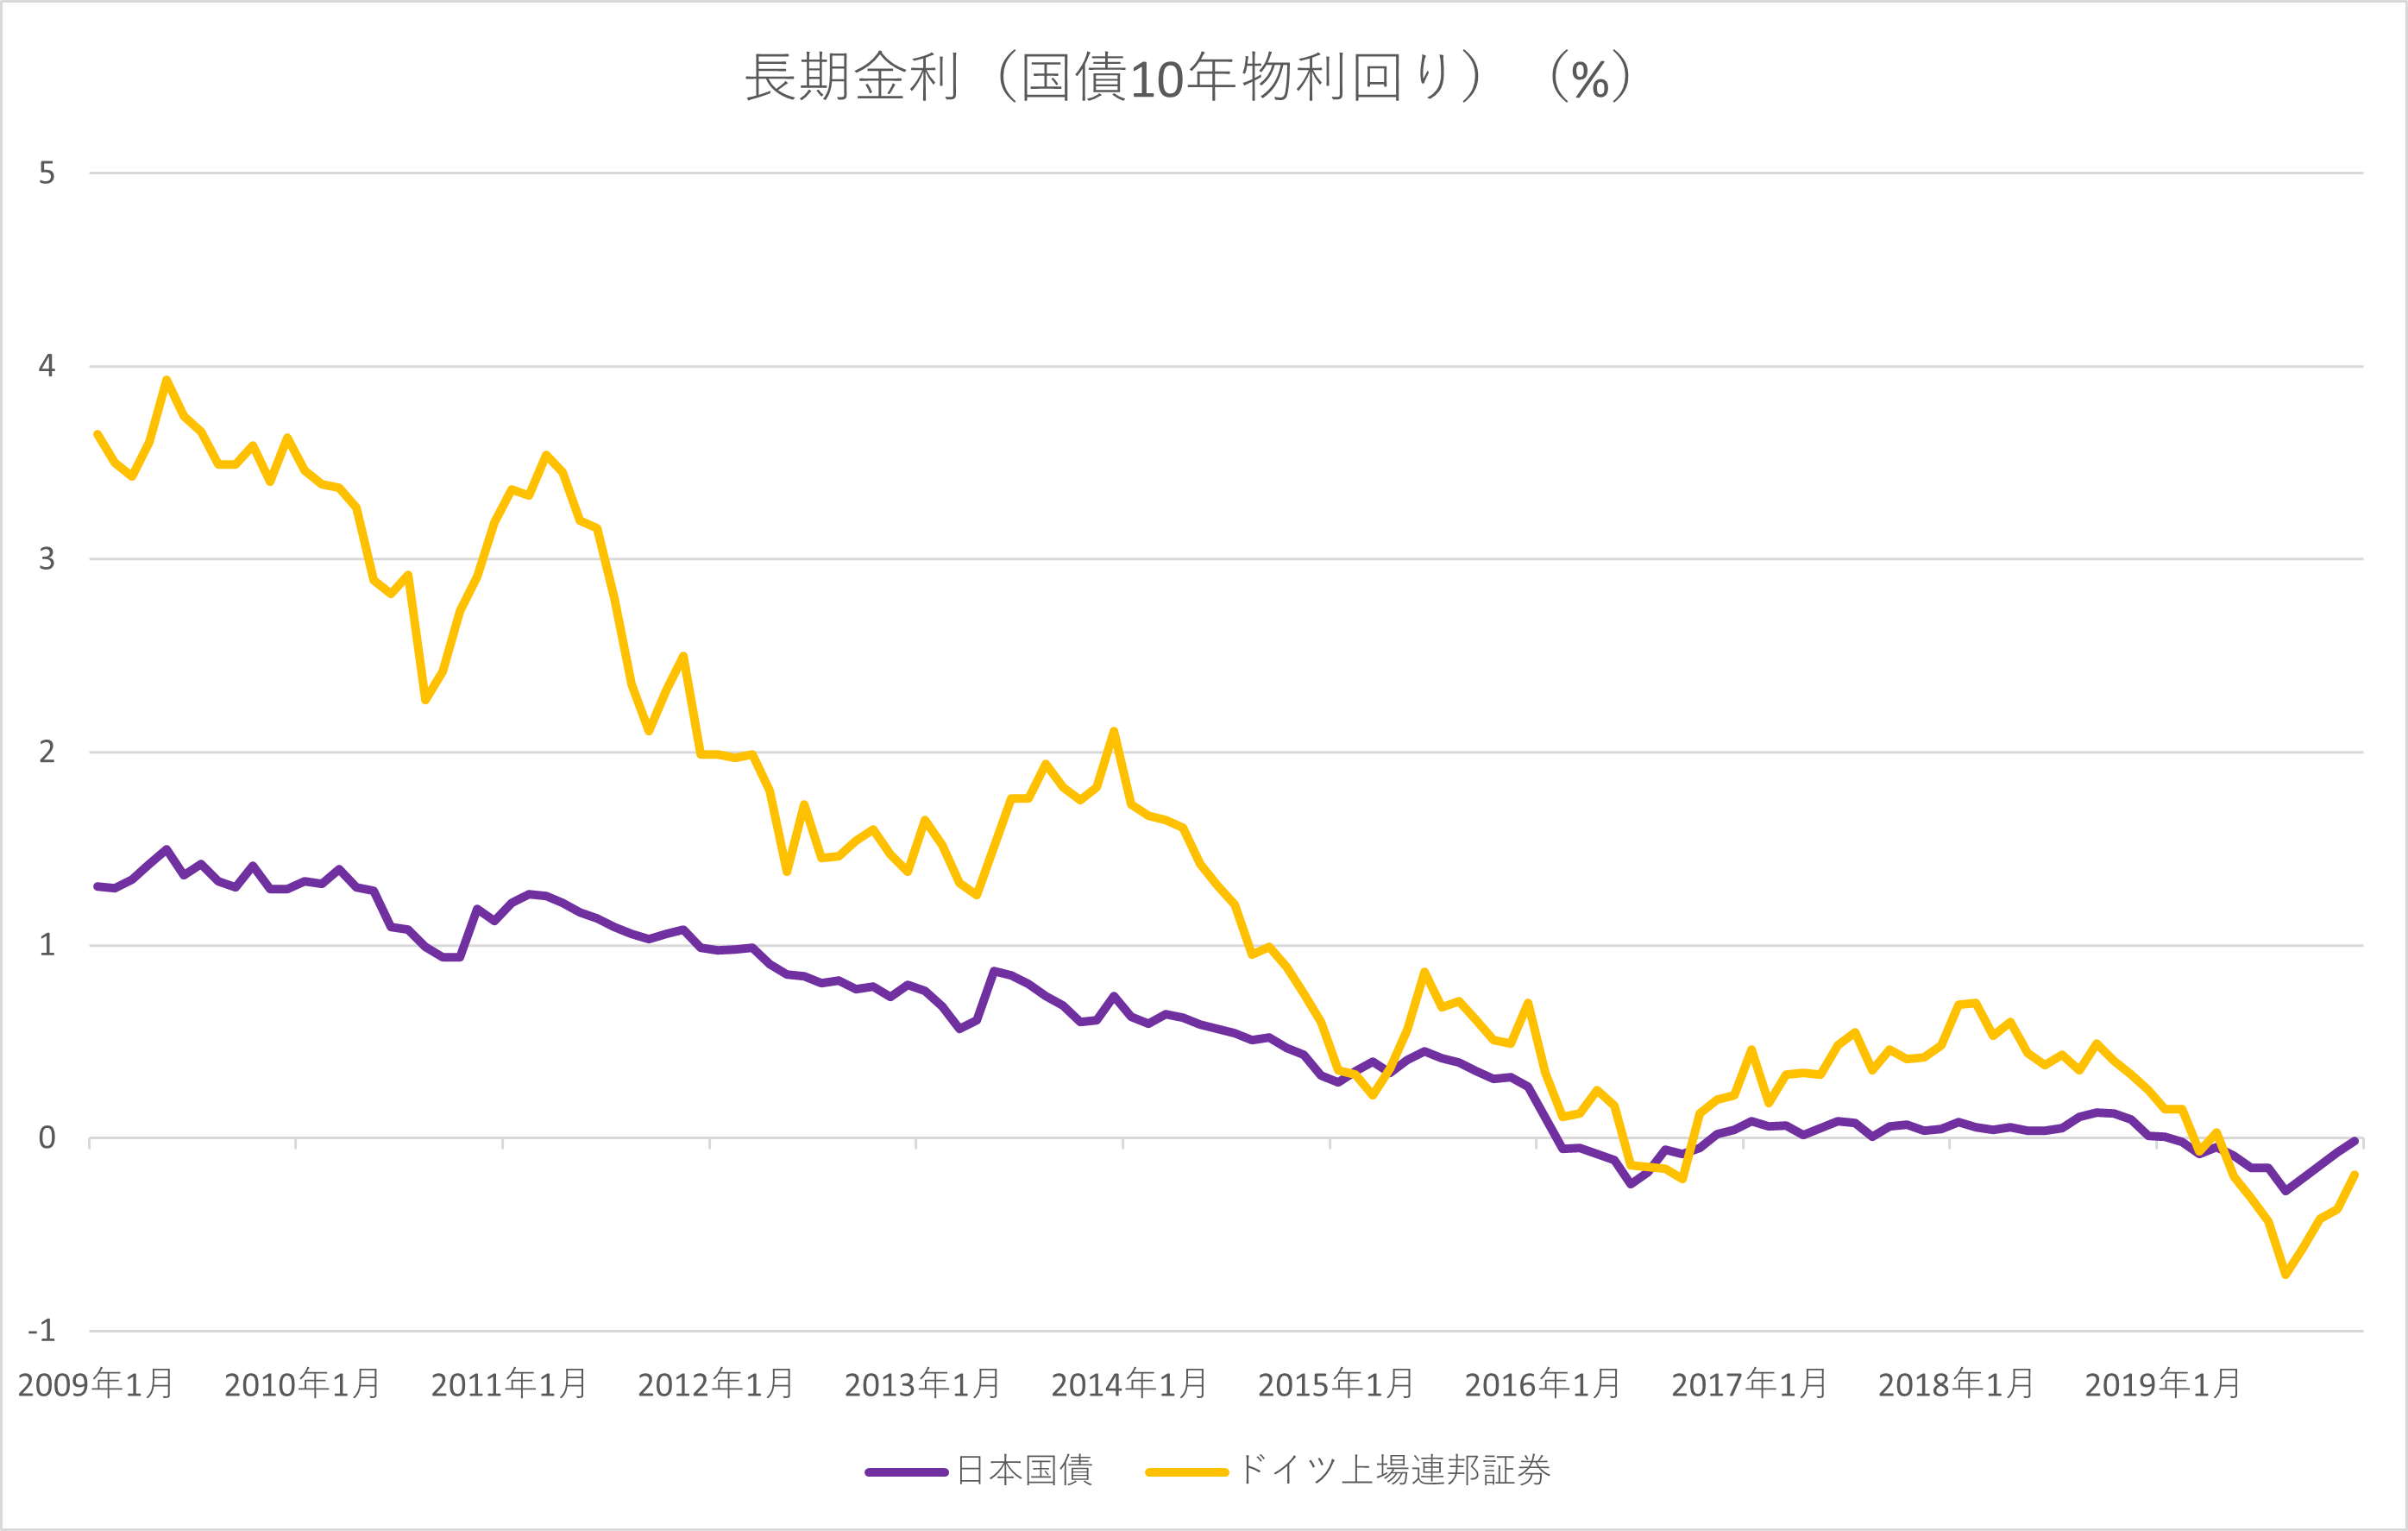
\includegraphics[width=16cm]{bond09.png}
\end{figure}
\newpage

\section{分析結果}

\subsection{Cholesky分解}

Cholesky分解を用いた構造型VARモデルを用いて推計を行った。変数の外生性の順は日本での分析においては$JMB$,$JLIBOR$,$JBOND$,$USDJPY$,$JSTOCK$,$JCPI$とし,欧州での分析においても同様に$EMB$,$ELIBOR$,$EBOND$,$USDEUR$,$ESTOCK$,$EHICP$である。本稿ではこの順序の変数の順序を用いたが,想定される他の変数の順序でも同様の結果が得られたため,本稿ではこの順序のものを記載している。
モデルに非定常な変数が含まれ,推計されたインパルス応答関数の信頼区間で有意であるとは言い切れない。しかし,今回の推計では有意性に大きく影響を及ぼさないと仮定し,95\%信頼区間を参考に,想定される波及効果について紹介する。

VAR分析の累積インパルス応答は以下の図に示してある。分析の結果,日本のデータでは以下の関係が存在することが示唆された。

\begin{enumerate}
  \setlength{\leftskip}{30pt}
  \item 日本のマネタリーベースの拡大はCPIを上昇させる。
  \item 日本のマネタリーベースの拡大は長期金利を引き下げる。
  \item 日本のマネタリーベースの拡大は円安を引き起こし,株価の上昇に波及する。
\end{enumerate}

分析結果1より,マネタリーベースの拡大がCPIを上昇させる効果は確からしい。また,分析結果2の金融緩和政策が長期金利を引き下げる効果はWright [2011]をはじめとする先行研究とも一致する。分析結果3の円安を引き起こし,株価の上昇に貢献する効果についてもHonda et al. [2013]などで確認されている金融緩和の波及経路である。

円安や株価の上昇を波及経路としてCPIを上昇させていることが図より示唆されるが,いずれもCPIへの直接の影響を示す累積インパルス応答からは,波及経路を特定できたとは言い難い。
また,長期金利の低下も金融緩和政策の波及経路として想定されたものであるが,この分析からその効果は確認されなかった。

\newpage
\begin{figure}[!htbp]
  \caption{日本のデータでの構造型VARモデルのインパルス応答}
  \begin{center}
    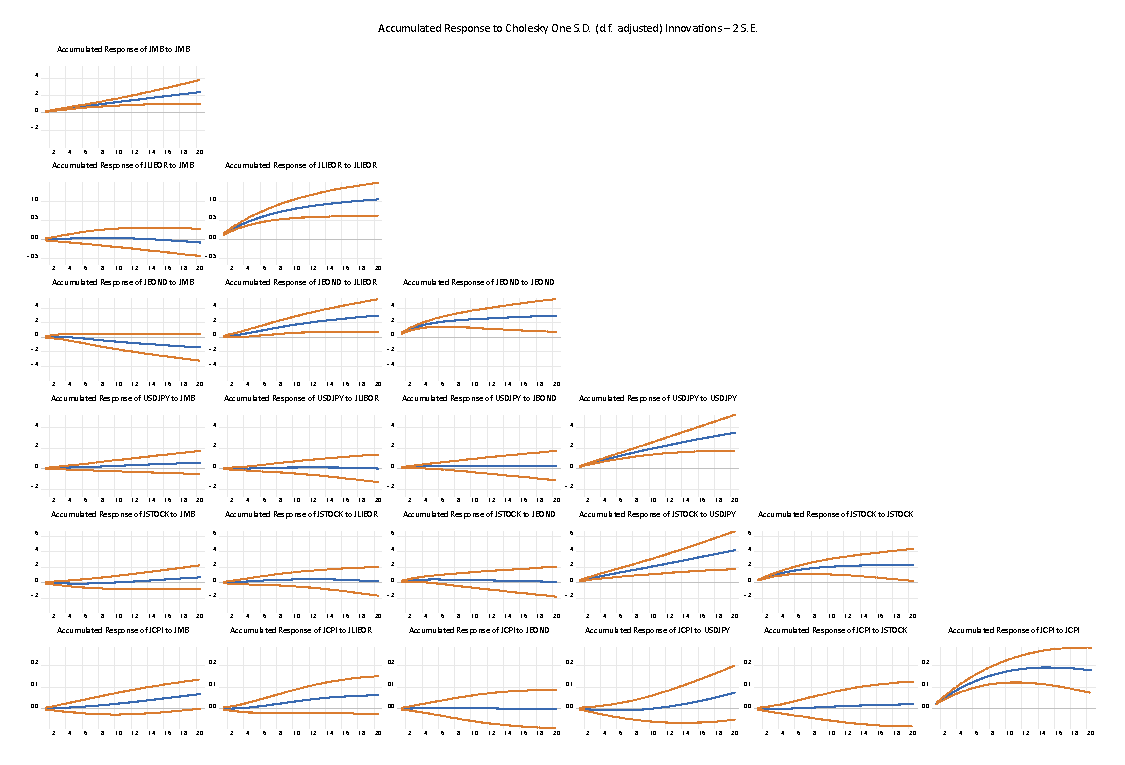
\includegraphics[width=18cm]{jimpulse.pdf}
  \end{center}
\end{figure}

\newpage
\begin{figure}[!htbp]
  \begin{minipage}{0.5\hsize}
    \caption{長期金利のインパルス応答}
    \begin{center}
      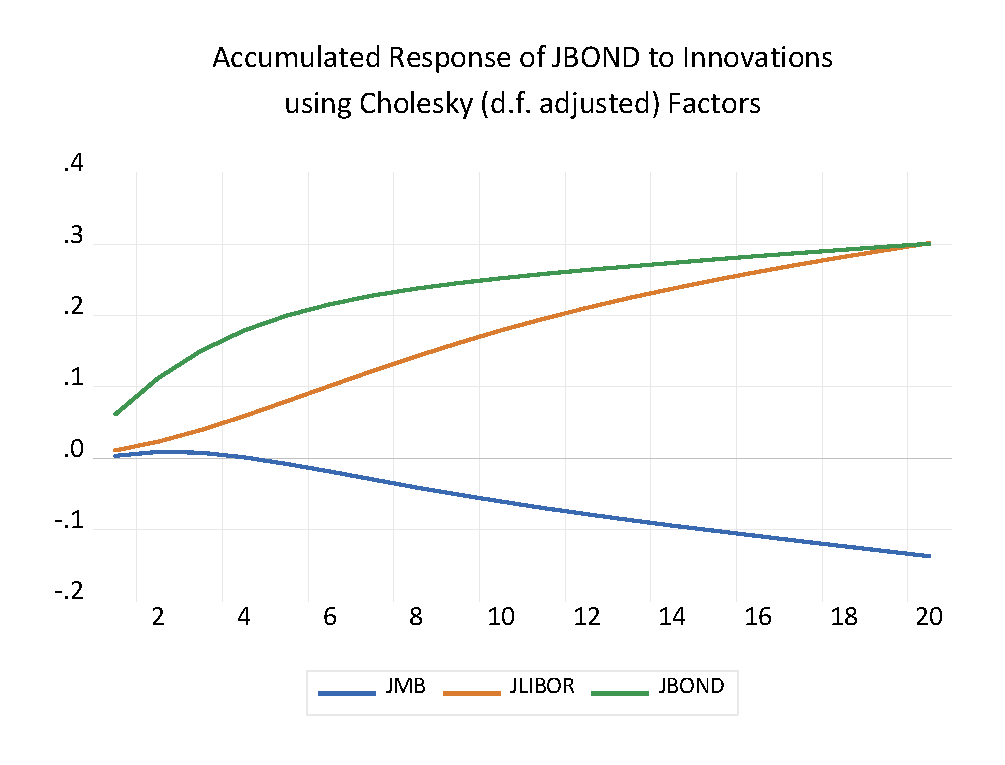
\includegraphics[width=9cm]{ijbond.pdf}
    \end{center}
  \end{minipage}
  \begin{minipage}{0.5\hsize}
    \caption{為替レートのインパルス応答}
    \begin{center}
      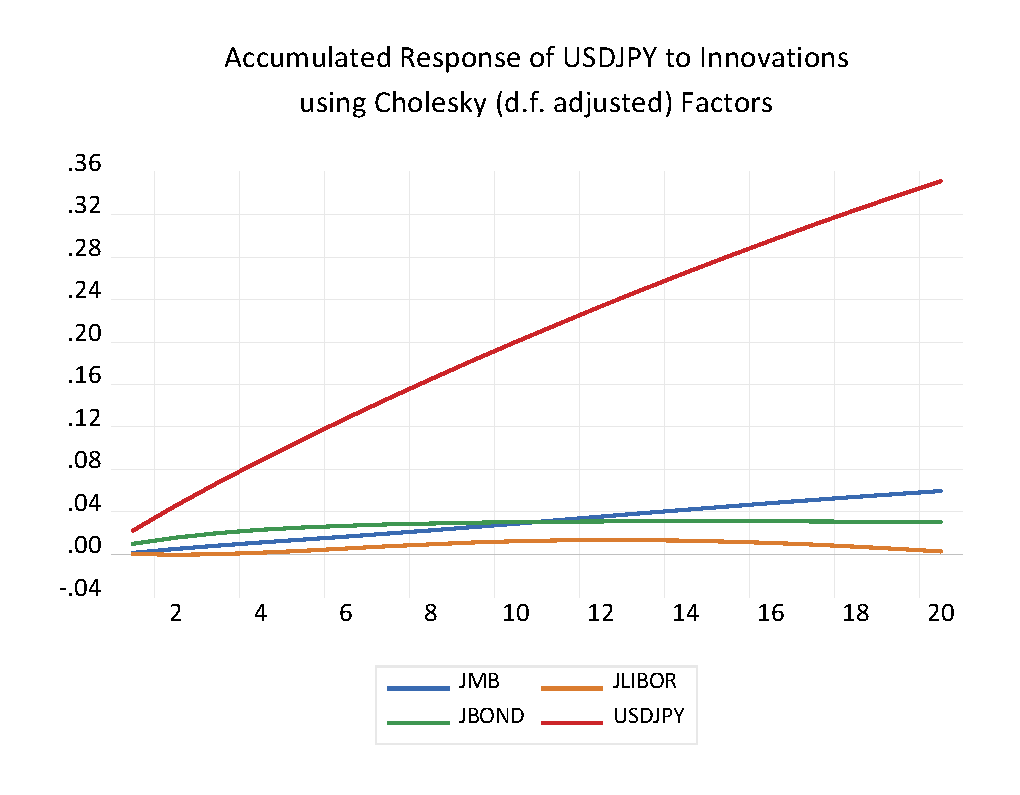
\includegraphics[width=9cm]{ijrate.pdf}
    \end{center}
  \end{minipage}
  \begin{minipage}{0.5\hsize}
    \caption{株価のインパルス応答}
    \begin{center}
      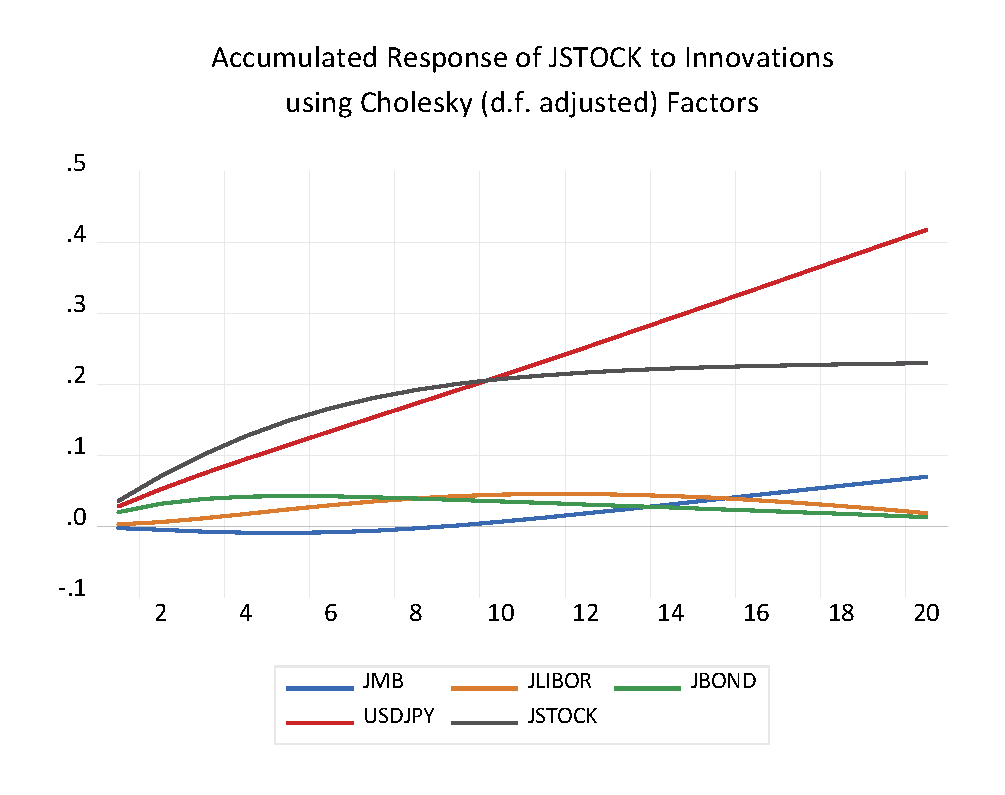
\includegraphics[width=9cm]{ijstock.pdf}
    \end{center}
  \end{minipage}
  \begin{minipage}{0.5\hsize}
    \caption{CPIのインパルス応答}
    \begin{center}
      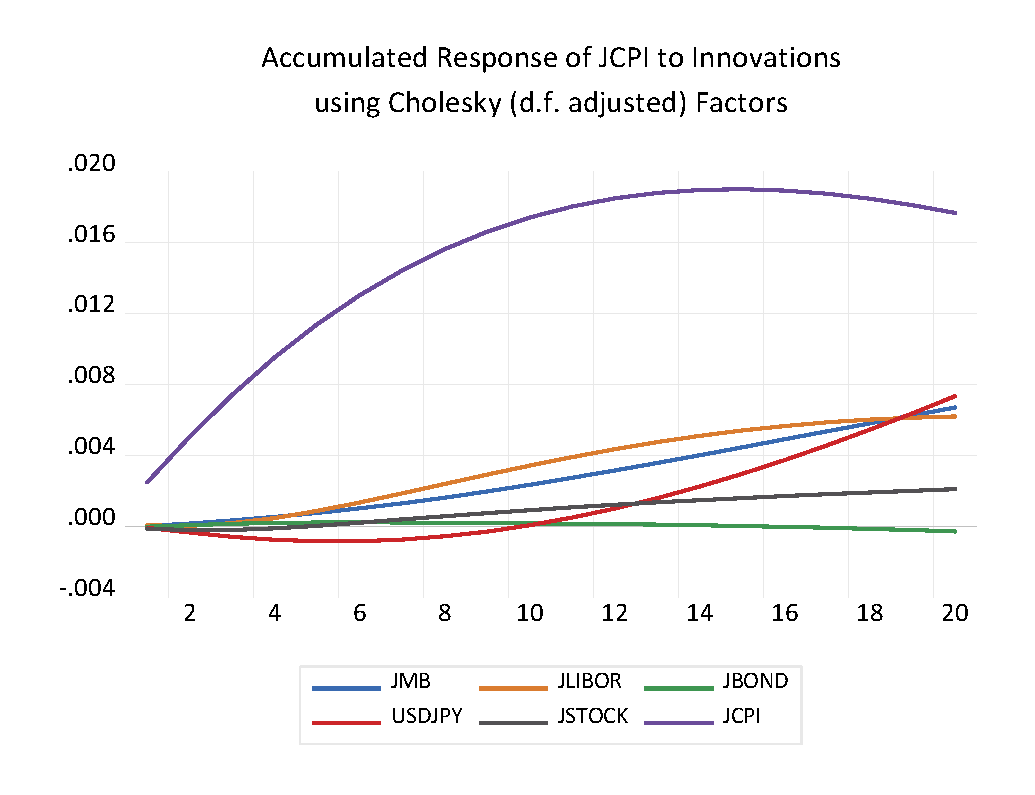
\includegraphics[width=9cm]{ijcpi.pdf}
    \end{center}
  \end{minipage}
\end{figure}

\newpage

次に欧州のデータでは以下の以下の関係が存在することが示唆された。
VAR分析の累積インパルス応答は以下の図に示してある。

\begin{enumerate}
  \setlength{\leftskip}{30pt}
  \item 欧州のマネタリーベースの拡大はHICPを上昇させる。
  \item 欧州のマネタリーベースの拡大は短期金利を引き下げ,株価の上昇に波及する。
  \item 欧州のマネタリーベースの拡大はユーロ安を引き起こし,株価の上昇に波及する。
  \item 欧州の株価の上昇はHICPの上昇に波及する。
\end{enumerate}

欧州でも日本と同様に金融緩和政策がマネタリーベースの拡大がCPIを上昇させる効果は確からしいことが分かった。また,自国通貨安を引き起こし,株価を上昇させる効果についても同様である。
累積インパルス応答からも,欧州では自国通貨安とそれによって起こる株価の上昇が物価上昇に影響していた可能性が高く,金融緩和政策の波及経路であることが示唆される。

また,日本のデータでは見られなかった短期金利の引き下げ効果とそれの株価への波及が見られる。
一方で,Pazicky [2018]などで確認されている時間軸効果による長期金利の低下は見られなかった。

\newpage
\begin{figure}[!htbp]
  \centering
  \caption{欧州のデータでの構造型VARモデルのインパルス応答}
  \vspace{10pt}
  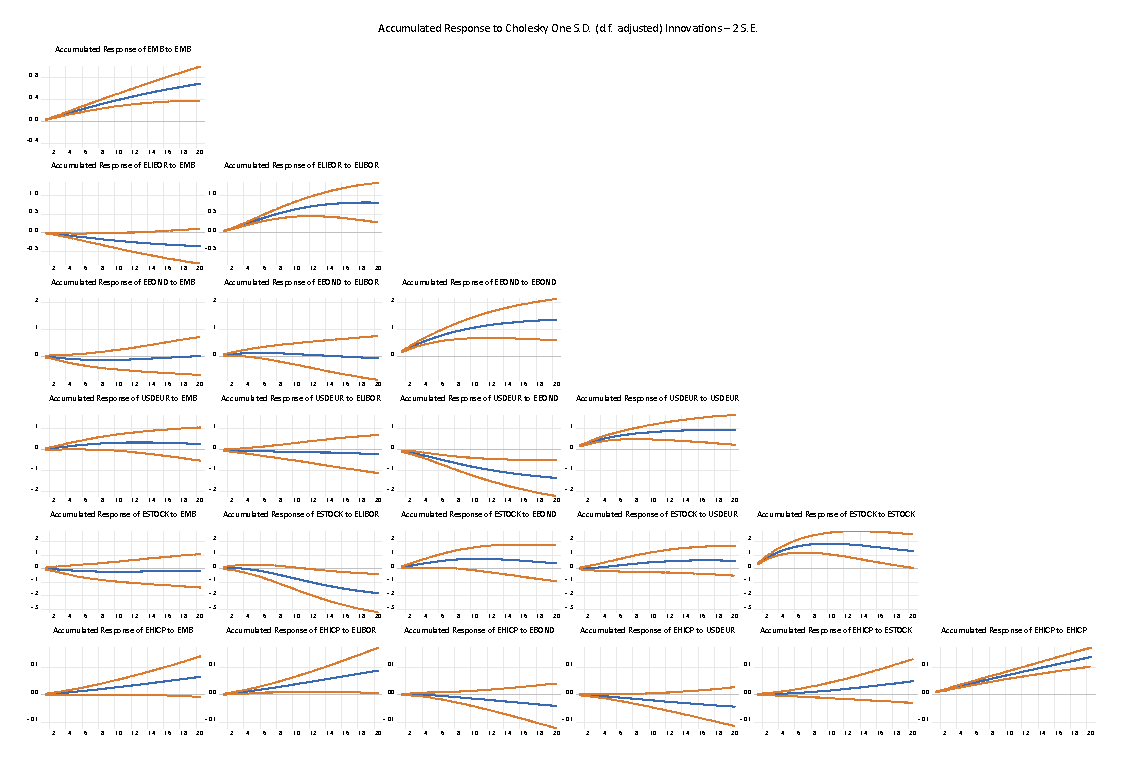
\includegraphics[width=18cm]{eimpulse.pdf}
\end{figure}

\newpage
\begin{figure}[!htbp]
  \begin{minipage}{0.5\hsize}
    \caption{短期金利のインパルス応答}
    \begin{center}
      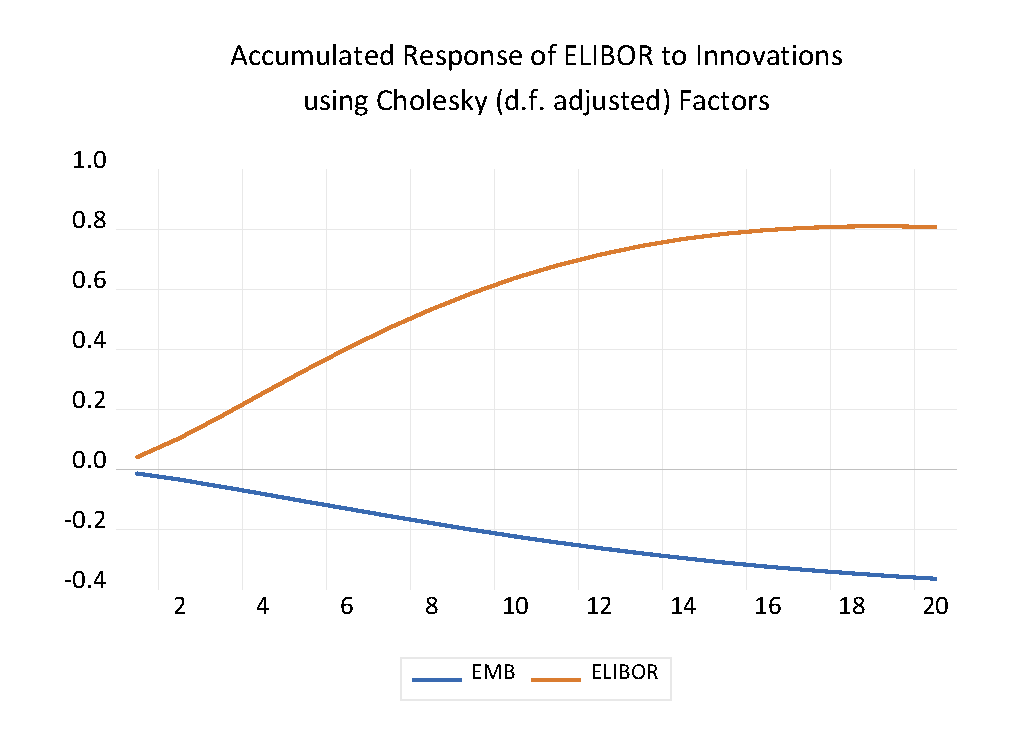
\includegraphics[width=9cm]{ielibor.pdf}
    \end{center}
  \end{minipage}
  \begin{minipage}{0.5\hsize}
    \caption{為替レートのインパルス応答}
    \begin{center}
      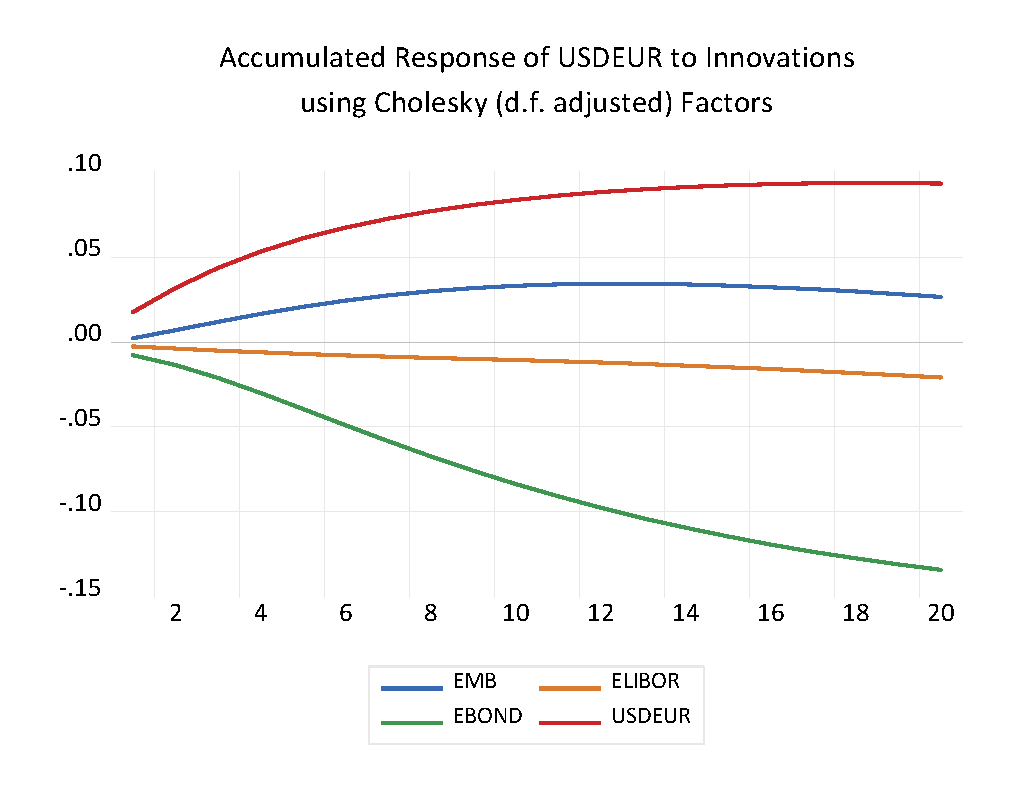
\includegraphics[width=9cm]{ierate.pdf}
    \end{center}
  \end{minipage}
  \begin{minipage}{0.5\hsize}
    \caption{株価のインパルス応答}
    \begin{center}
      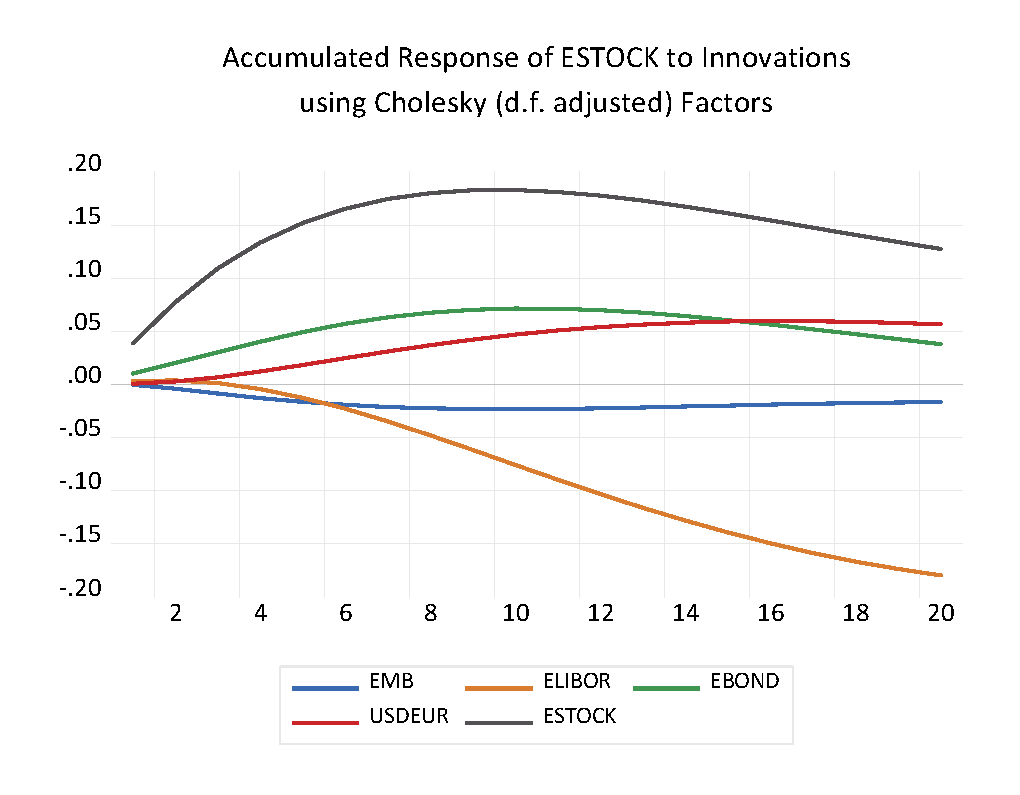
\includegraphics[width=9cm]{iestock.pdf}
    \end{center}
  \end{minipage}
  \begin{minipage}{0.5\hsize}
    \caption{HICPのインパルス応答}
    \begin{center}
      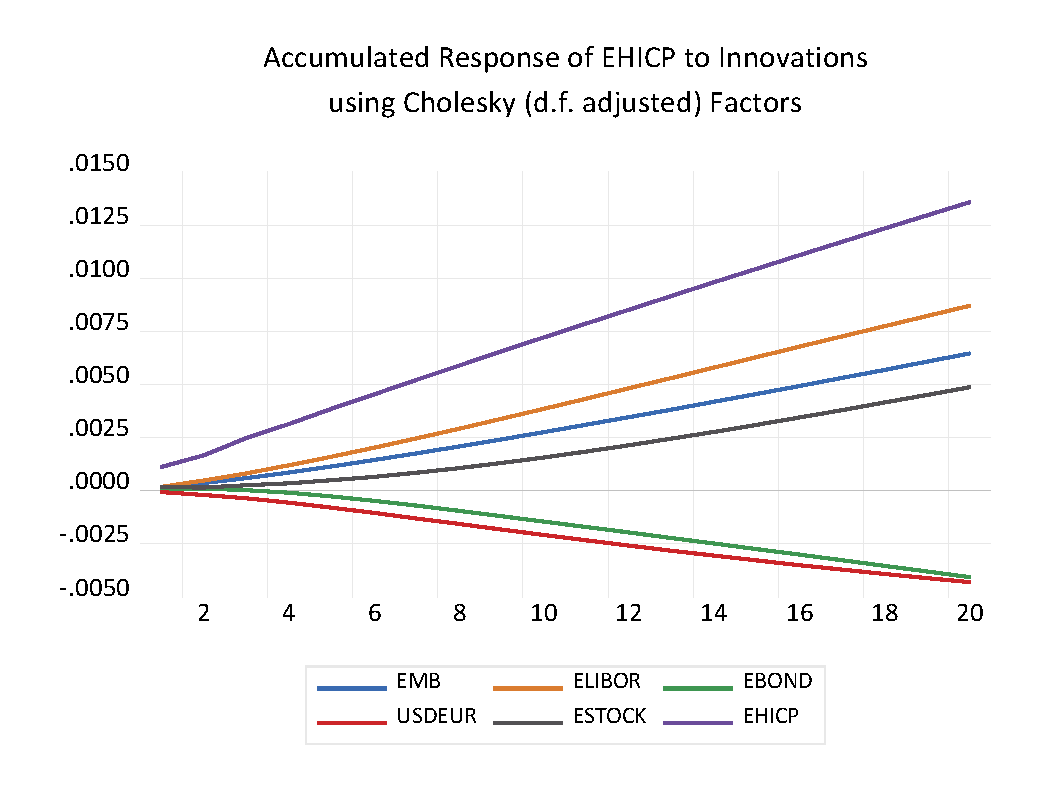
\includegraphics[width=9cm]{iehicp.pdf}
    \end{center}
  \end{minipage}
\end{figure}

\newpage
\subsection{重回帰分析}

次に,日本銀行による物価目標へのコミットメントを行うアナウンスメントの物価への効果を測定するため,以下の出された時期の異なる2種類のアナウンスメントをダミー変数とし,その効果について重回帰分析を用いて測定した。

最初に,使用するデータのうち,$JLIBOR$,$JBOND$,$USDJPY$,$JCPI$に単位根過程がないかを調べるために単位根検定として拡張ディッキーフラー (ADF)検定を行った。
水準データでは$JLIBOR$のみ,単位根過程を棄却できた。
水準データで単位根過程を棄却できなかった$JCPI$,$JBOND$,$USDJPY$は差分を取ることで単位根過程を棄却できたため,差分を取って重回帰分析に使用した。
%%また,共和分検定はヨハンセンの手順で行い,共和分がないことを確認している。

差分系列への回帰を行う際,消費増税ダミー変数$TAXDUMMY$については一時的な物価上昇を考慮するためのものであるため,同じく差分を取って使用した。一方で,政策アナウンスメントダミー変数$ITDUMMY$,$OSDUMMY$については一時的な影響ではなく,今後の物価の上昇率に影響を与え続けるものと仮定し,差分を取らずに使用する。

まず,日本の物価安定目標2\%のインフレターゲットの導入前後での変化について重回帰分析を行った。
分析の結果,政策ダミー変数 ($ITDUMMY$)は正に有意となった。詳細な結果は図13のとおりである。

次に,強力な金融緩和継続のための枠組み強化として出された「オーバーシュート型コミットメント」導入前後での変化について同様の重回帰分析を行った。分析の結果,政策ダミー変数 ($OSDUMMY$)の係数は負で有意性が確認されなかった。詳細な結果は図14のとおりである。

\newpage
\begin{figure}[!htbp]
  \centering
  \caption{インフレターゲット導入での重回帰分析の結果}
  \vspace{5pt}
  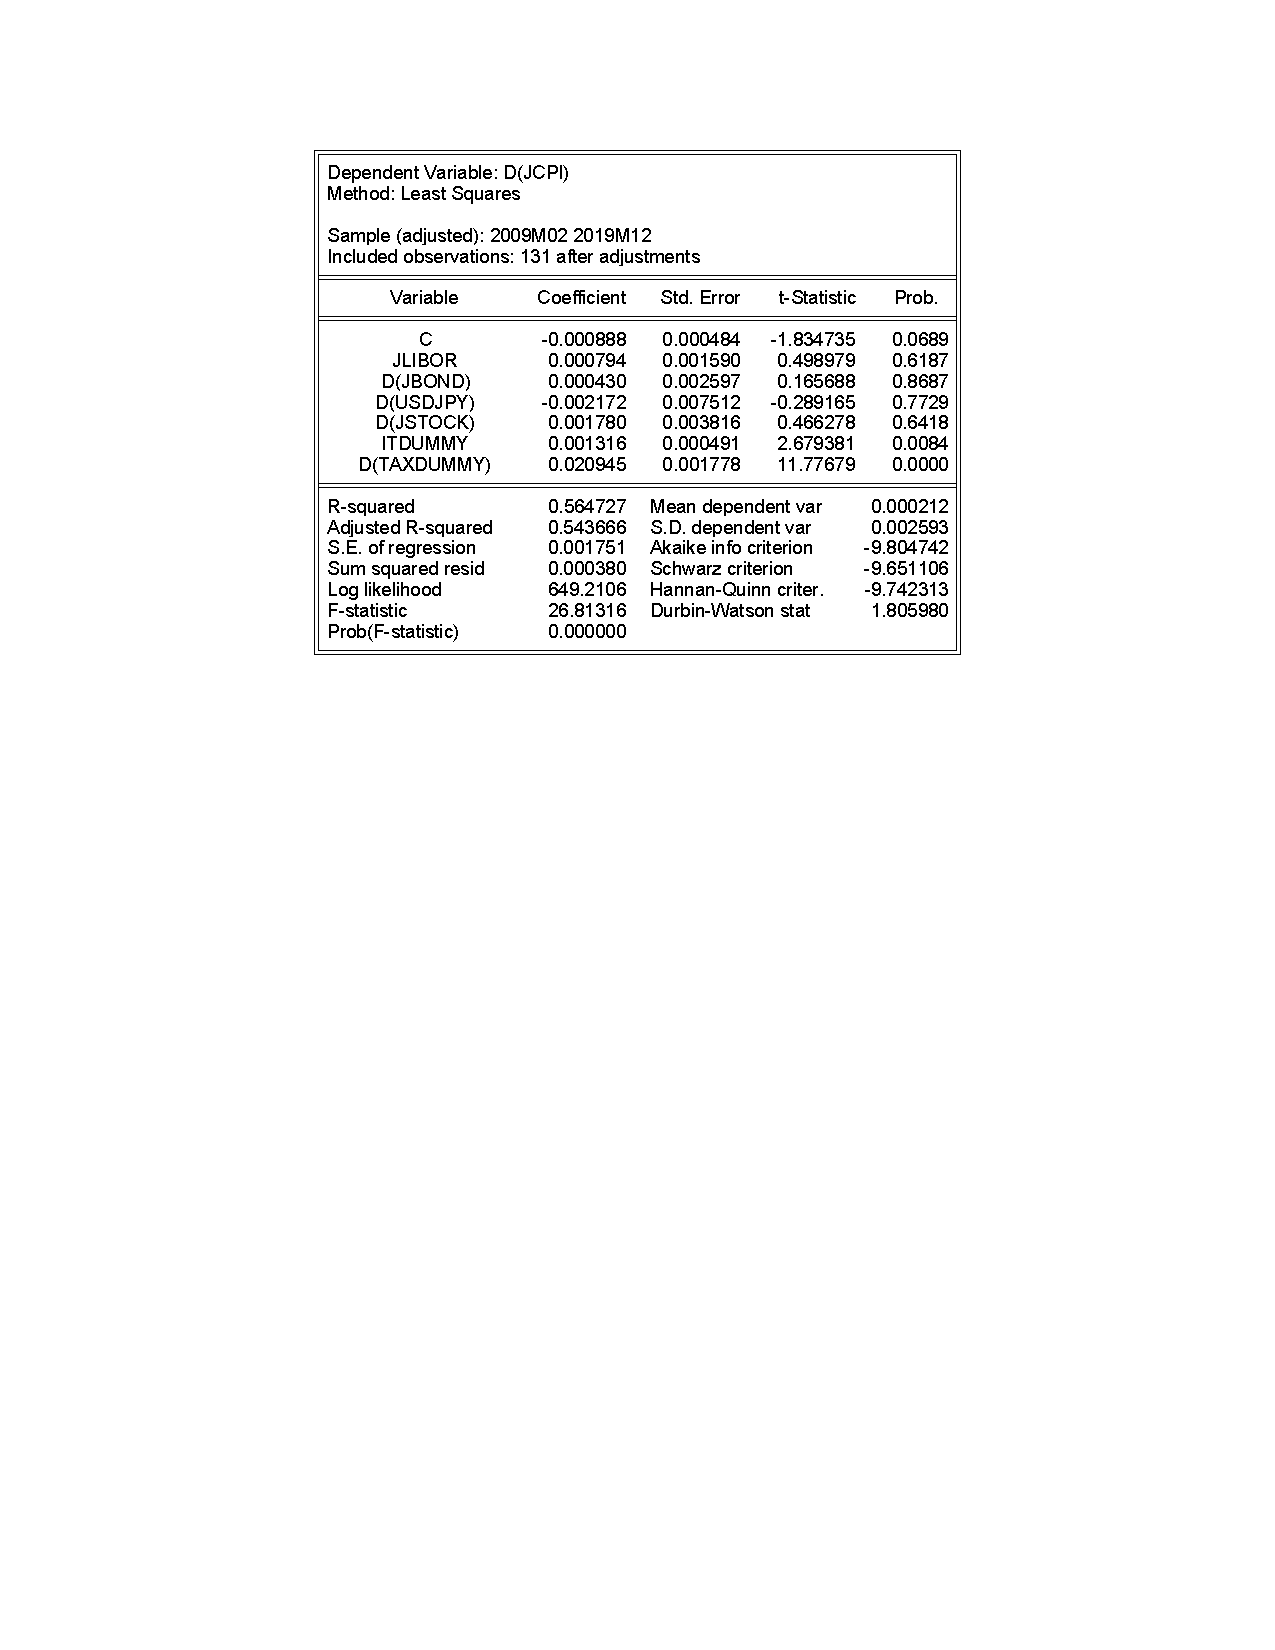
\includegraphics[width=12cm]{it.pdf}

  $ITDUMMY$は5\%有意水準で帰無仮説が棄却される。
\end{figure}

\begin{figure}[!htbp]
  \centering
  \caption{オーバーシュート型コミットメント導入での重回帰分析の結果}
  \vspace{5pt}
  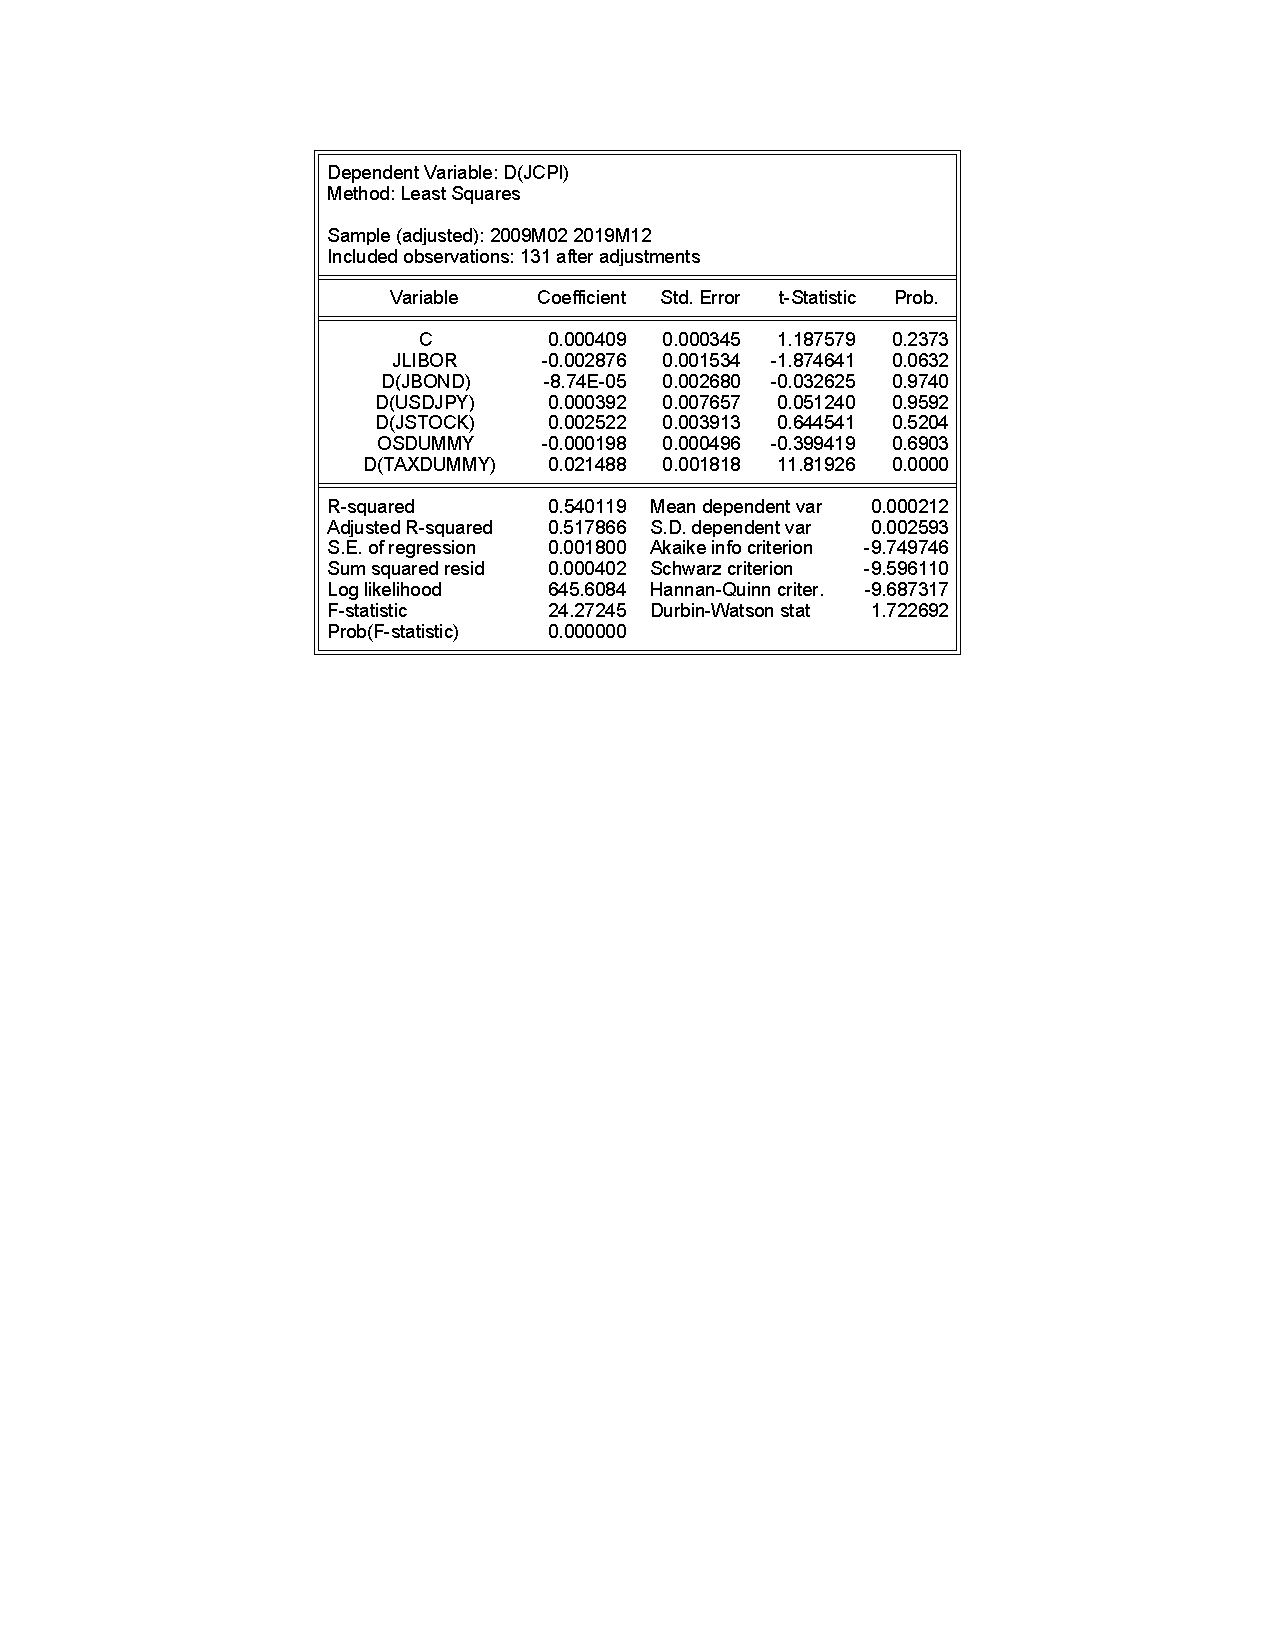
\includegraphics[width=12cm]{os.pdf}
\end{figure}

%日本での分析結果では長期金利の低下や円安の進行が物価上昇に有意に影響を与えたと確認され,日本銀行の「オーバーシュート型コミットメント」についても物価上昇に対し,有意な影響があったと言える。
%日本銀行は2013年1月に初めて,物価安定目標2\%を定めているが,それから3年以上後のアナウンスメントでも,再度コミットメントを行うことで効果が見られたというのは興味深い結果である。
%生鮮食品を除く消費者物価指数 (コアCPI)の前年比上昇率の実績値が安定的に2%を超えるまで,マネタリーベースの拡大方針を継続するというコミットメントが物価目標に対する国民の一定の信認を得られているということが判明したことも大きい。
%影響の大きさとしては円安の進行によるものが大きく,円安による輸入物品の物価上昇などの影響は大きく反映されている可能性が高い。一方で,株価からの影響については負で有意でないものになっており,円安の進行によって輸出が拡大し,株価が上昇するというシナリオは機能しなかったと考えられる。

%欧州のデータでは長期金利と政策ダミーについて日本と同様の結果になったのに対し,為替レートと株価からの影響については逆の結果が見られた。
%株価の上昇が物価上昇をもたらすことについては金融緩和政策の将来の価格上昇への期待を高めるというのに合致しているが,ユーロ高の際に物価が上昇するという影響については不自然である。これについては,ユーロ安と物価上昇について負の有意な関係かつ,株価からの影響よりも大きい効果が検出されているため,説明が難しい。
%また,政策ダミーについてはECBは量的緩和と同時に物価目標を導入しており,当時市場に衝撃を与えたことからも大きくを信認を得られたと考えることができる。

%以上のように,日本と欧州の両方において,主な変動要因には先の構造型VARモデルでの分析結果との整合性が見られる。また,物価目標へのコミットメントについては日本と欧州でアナウンスメントを行った状況やタイミングが異なる一方で,ほとんど同じ効果が見られた。物価上昇に対して,有意な生の影響が確認されることからも金融緩和の方針転換や追加の際にアナウンスされる物価目標へのコミットメントは金融緩和の効果を高めることにおいて,十分に効果を発揮していると考えられる。


\newpage

\subsection{分析結果の考察}

Cholesky分解を用いた構造型VARモデルの推計結果を考察すると,日本と欧州の両方で,マネタリーベースの拡大が物価を上昇させる効果が示唆された。
したがって,マネタリーベースの拡大は何らかの経路で物価に波及している可能性が高い。

日本のデータの分析からはマネタリーベースの拡大が長期金利を低下させる時間軸効果が働いていることが確認できる。
また,円安を引き起こし,それが株価の上昇に波及する効果も確認されており,これらが波及経路である可能性が高いが,いずれもインパルス応答からはCPIへの効果は確認できず,波及経路であるということは難しい。

一方で,欧州のデータの分析からは日本と同様のユーロ安を引き起こし,それが株価の上昇に波及する効果が確認された。さらに株価の上昇がHICPに正の影響を与えることが確認されており,これが金融緩和政策の波及経路となっている可能性が高い。
また,短期金利の引き下げ効果がみられることについては,データ期間である2009年から2019年の間にECBによる中銀預金金利の利下げが複数回,マネタリーベースの拡大と並行して行われており,これが強く反映されている可能性が高い。
そして,短期金利の低下から株価の上昇への波及が見られることについては,ECBによる追加の利下げがフォワード・ルッキングな期待形成につながったことが示唆される。
この期待形成が株価の上昇を通して物価に対して正の影響を与えた可能性が高いと評価できる。

また,日本のデータを用いた重回帰分析の結果を考察すると,2013年1月に出されたインフレターゲット導入のアナウンスメントは,CPIに対して有意な正の影響をもつことから,フォワード・ルッキングな期待形成を行うことができたと考えられる。この時期は「量的・質的金融緩和」が開始される3ヶ月前であり,将来の追加緩和の可能性を予測しやすい状況であったことも大きく影響している可能性が高い。

一方で, 「オーバーシュート型コミットメント」導入のアナウンスメントはCPIに対する有意な影響が確認されなかった。これはすでに「マイナス金利付き量的・質的金融緩和」が行われているにもかかわらず,景気回復が行われていないため,適合的な期待形成が行われたことに起因すると考えられる。

したがって,物価目標へのコミットメントを行うアナウンスメントの効果はフォワードルッキングな期待形成が行われやすい状況下,例えば大規模な金融緩和政策の開始前などでは物価への影響をもつものの,近年のようにすでに大規模な金融緩和政策が行われている状況下では効果をほとんど持たないと思われる。
%現在,日本銀行やECBが物価目標へのコミットメントを行うアナウンスメントを行った場合,物価に対する影響は見られない可能性が高い。

%Cholesky分解を用いた構造型VARモデルの推計結果を考察すると,2013年から2018年までの全期間のデータでの分析では長期金利の低下が金融緩和政策の物価への波及経路として示唆された。しかしながら,非マイナス金利政策期のみのデータを用いた分析においては長期金利の低下はCPIを上昇させる効果は有意ではなく,マイナス金利政策期のみのデータを用いた分析ではマネタリーベースの増加が短期金利と長期金利を引き下げる効果が有意ではない。

%一方,同時点間の影響についてのより精密な分析である金融政策ショックの識別を用いた構造型VARモデルでの推計結果では,マネタリーベースの拡大が長期金利の低下をもたらす効果について頑健性が確認された。
%したがって,マイナス金利政策期においてもマネタリーベースと長期金利の関係性が存在すると考えられ,マイナス金利期でのCholesky分解において有意な結果が得られなかったことにはマネタリーベースの拡大以外の要因による長期金利の変動が影響した可能性が高い。図1より2016年2月を境に長期金利は大きく低下している一方,マネタリーベースはそれより緩やかに上昇している。このことよりマイナス金利政策の開始以降は日銀当座預金の超過準備へのマイナス金利の付利が長期金利の低下に大きく影響したと考えられる。

%以上より,金融緩和政策による物価上昇への効果は確認されるものの,その波及経路については有意な結果が出なかったため不明である。
%長期金利の低下は非マイナス金利政策期での分析において有意な結果が得られなかったことから,2013年から始まったQQEの波及経路ではない可能性が高い。一方,マイナス金利政策期においては金融緩和政策ではなく,マイナス金利政策やイールドカーブ・コントロールによって長期金利が引き下げられていると考えられる。また,この期間においては長期金利の低下が物価上昇へ正の影響を与えることが確認されることから,長期金利の低下は2016年から始まったマイナス金利政策の波及経路である可能性が高い。

\newpage
\section{結論}

本稿はCholesky分解を用いた構造型VARモデルでの金融緩和政策の波及経路の分析と,重回帰分析による物価目標のコミットメントを行うアナウンスメントの効果の測定により,今後,中央銀行がとるべき金融緩和の方針や追加緩和のあり方を考察するものである。

日本の量的・質的金融緩和が物価に与えた影響を分析した論文は非常に少なく,第2章で紹介した矢野・岡田 [2018],宮尾 [2016]や日本銀行の公式見解のほかには知られていない。
また,欧州の量的金融緩和政策が物価に与えた影響を分析した論文としてはPazicky [2018]が詳しいが,ECBによる開始が2015年と比較的最近であることからも分析した論文は少ない。
これらの先行研究ではその波及経路について触れられており,矢野・岡田 [2018]では為替レートやインフレ予想,Pazicky [2018]では時間軸効果による長期金利の低下が波及経路として挙げられている。

本稿ではこれらの論文と同様のCholesky分解を用いた波及経路の特定に加え,日本と欧州の異なる状況下での波及を比較することで,双方で示唆された波及経路についての頑健性を確認するとともに,双方で異なる波及経路についてその要因分析を行っている。

まず,本稿の構造型VARモデルでの分析においては為替レートを通した経路が金融緩和政策の波及経路として最も有力であるという結果になった。
これについてはマネタリーベースの拡大が自国通貨を減価させる影響を持つことが日本と欧州の両方で確認されていることから金融緩和政策の効果としては有効なものである可能性が高いと言える。
自国通貨の減価は輸入物品の価格上昇を通して,物価の上昇に波及することが多くの先行研究で確認されており,
実際に本稿における欧州の分析ではユーロ安の物価への波及も確認されることから一定の政策効果もあったと思われる。
一方,日本の分析で物価への波及が確認されなかった理由としては,欧州と比べて日本の物価の上昇が僅かであることなどが考えられるが,詳細については輸入物品と非輸入物品の価格の変動について精査する必要がある。

金融緩和の波及経路については時間軸効果による長期金利の低下などが特に有名であるが,本稿では日本での分析において,マネタリーベースが時間軸効果によって,長期金利を低下させる効果が見られただけに過ぎず,物価への波及も見られないことから物価への効果としては大きいものではない可能性が高い。
一方で,短期金利については特に欧州のデータで大きな低下があり,これが株価の上昇を通じて物価上昇に波及している。これはフォワード・ルッキングな期待形成により,将来の資産価格上昇への期待が高まったことが要因である。
短期金利の低下がECBによる中銀預金金利の利下げの影響であることは前述のとおりであるが,具体的には2014年9月 (▲0.2\%),2015年12月 (▲0.3\%),2016年3月 (▲0.4\%),2019年9月 (▲0.5\%)の4回の利下げが行われている。
これは2014年6月 (▲0.1\%)以来,利下げのない日本と比べて,格段に多い利下げの幅と回数である。

以上の波及経路の考察より,金融緩和政策による物価目標の達成のためには自国通貨安への誘導が効果的であるという結果になった。
現在,各国の中央銀行,特に日本銀行は時間軸効果に期待して,「イールドカーブ・コントロール」など,長期金利の誘導を目標に掲げているが,目標為替レートを公開する方が効果的であるかもしれない。
また,欧州のデータの分析結果からは政策金利の利下げも有効であるように思われるが,これはデメリットも強いものである。
特に日本では政策金利の利下げによる民間銀行の収支の悪化が顕著であり,判断が難しくなっている。
欧州でも既に▲0.5\%まで利下げが行われていることから,利下げの余地が多く残されているとは言えず,今後の追加緩和案として一概に有用なものとは言えない。

また,物価目標に関するアナウンスメントの効果を測定した重回帰分析では,2013年のアナウンスメントが物価上昇への効果があった一方で,2016年のアナウンスメントは有意な効果が認められないという結果になった。このことから,金融緩和政策の開始初期ではフォワード・ルッキングな期待形成が行われやすいが,金融緩和政策が長期化するのにつれて適合的な期待形成がなされるようになり,アナウンスメントの効果が逓減すると考えられる。
この物価目標については特にECBが現在,見直しを検討しており,アナウンスメント効果についても期待しているものと思われる。しかし,本稿の分析の結果からは,仮に物価目標の見直しとアナウンスメントが行われた場合にも物価への影響はほとんどないように思われる。

以上のことを踏まえると,金融緩和が長期化している現在,追加の緩和で効果を出すのは困難であると思われる。
政策金利の利下げについては効果も大きいが,デメリットも多い諸刃の剣であることがよく言われるほか,さらなる利下げの余地もほとんど残されていない。
また,ECBが検討中の物価目標の見直しなどの期待形成への働きかけも,適合的な期待形成によって物価上昇などには波及しないことが見込まれるため,これに効果を見出すのは現実的ではない。
しかしながら,為替レートの自国通貨の減価は輸入物価の上昇による物価への影響を期待できるため,比較的効果があるように思われる。
現在,各国の中央銀行はあまり為替レートの変動を考慮にいれていないように思われるが,為替レートの目標値を公開するなどのアプローチを取れば,金融緩和の効果を向上できる可能性がある。


%本稿は日本銀行の金融緩和政策の物価上昇への効果について,2013年から2018年の日次データによって,Cholesky分解と金融政策ショックの識別の2種類の構造型VARモデルで分析したものである。

%現在,日本のQQEが物価に与えた影響を分析した論文は少なく,先行研究として紹介した矢野・岡田 (2018),宮尾 (2016)や日本銀行の公式見解のほかにはあまり知られていない。本稿ではこれらと同様のCholesky分解によって波及経路の特定を試み,また,金融政策ショックの識別も行うことで結果の頑健性を確認した。矢野・岡田 (2018)では為替レートやインフレ予想が波及経路として考えられるとされたが,本稿の分析においては為替レートは波及経路としては考えにくいという結果になった。また,金融緩和政策自体の波及経路については特定ができなかったが,2016年からのマイナス金利政策の波及経路については明らかになったと言える。

%日本銀行のマイナス金利政策は日銀当座預金の超過準備に▲0.1\%のマイナス金利が適用されるものであり,これにより銀行間の取引金利である短期金利も引き下げられる。短期金利の低下は長期金利を低下させ (分析結果3),長期金利の低下はCPIを上昇させる (分析結果7)。

%つまり,2016年2月以降のマイナス金利政策は物価上昇に寄与しており,またその波及経路は長期金利であるため,同年9月に開始されたイールドカーブ・コントロールは物価安定目標2\%の達成に向けた政策として効果があったと考えられる。

%QQEの開始から約7年が経とうとしているが,2\%の物価安定目標は達成されておらず,日本銀行が2019年10月に公表した「経済・物価情勢の展望」の中でも2021年度のコアCPIの前年比の見通しが1.6\%上昇であることからも先行き不安が残る結果となっている。しかしながら,本稿の分析からは日本銀行がこれまでに行った金融緩和政策とそれに伴うイールドカーブ・コントロールは方向性を間違ったものではないと言える。このことからも日本銀行は長短金利は現在の低い水準を維持し,必要であればさらなる金利の引下げ「マイナス金利の深掘り」も選択肢に入れて安定目標の達成と持続を目指すべきである。

%日本銀行をはじめ,中央銀行が行う非伝統的金融政策の景気を刺激する効果はHonda et al. (2013)などでも明らかであるが,日本銀行の金融緩和が物価に与える影響,またその経路についての研究は少ない。本稿は日本銀行が行った金融緩和政策のCPIへの影響について日次データを用いて,より詳細な効果と波及経路について分析を行ったものである。

%分析結果は以下のとおりである。日本銀行の金融緩和政策による日銀当座預金残高の増加は確かにCPIに対して正の影響を与えている。これはCholesky分解と金融政策ショックの識別のいずれの結果においても頑健性が認められた。また,Cholesky分解の結果より金融緩和政策はマネタリーベースを拡大すると同時に長期金利の低下を引き起こし,これがCPIの上昇に寄与していることが示唆された。
%したがって,2016年9月より導入された「イールドカーブ・コントロール」には物価を上昇させる効果があり,適切な調節によって長期金利をコントロールすることで物価上昇を引き起こせる可能性がある。

\newpage

\addcontentsline{toc}{section}{参考文献}
\begin{thebibliography}{99}
  \bibitem{}  翁邦雄・白塚重典[2003]「コミットメントが期待形成に与える効果: 時間軸効果の実
  証的検討」金融研究第22巻第4号 pp.255-292
  \bibitem{} 翁邦雄[2017]「金利と経済: 高まるリスクと残された処方箋」ダイヤモンド社
  \bibitem{} 沖本竜義[2010]「経済・ファイナンスデータの計量時系列分析」朝倉書店
  \bibitem{} 柴本昌彦[2012]「日本の非伝統的金融政策ショックの識別と長短金利差への影響」国
  民経済雑誌第205巻第2号 pp.73-88
  \bibitem{} 白井さゆり[2016]「超金融緩和からの脱却」日本経済新聞出版社
  \bibitem{} 白塚重典・藤木裕[2001]「ゼロ金利政策下における時間軸効果:1999-2000年の短期
  金融市場データによる検証」金融研究第20巻第4号 pp.137-170
  \bibitem{} 照山博司[2001]「VAR による金融政策の分析:展望」『フィナンシャル・レビュー』
  第59号財務省財務総合政策研究所 pp.74-140
  \bibitem{} 内藤友紀[2017]「1930年代における日本の金融政策: 時系列分析を用いた定量的分
  析」関西大学出版部
  \bibitem{} 中澤正彦・矢野誠[2016]「金融危機後の公開市場操作のポートフォリオリバランス効果:
  買入長期国債の残存期間別データの構築による検証」MQ Discussion Series No.2015-005
  \url{http://www.market-quality.net/dp/2015-005.pdf} (2020年11月24日閲覧)
  \bibitem{} 日本銀行 [2016] 「『量的・質的金融緩和』導入以降の経済・物価動向と
  政策効果についての総括的な検証」(2016年9月21日) \url{https://www.boj.or.jp/announcements/release_2016/k160921b.pdf} (2020年11月24日閲覧)
  \bibitem{} 日本銀行 [2019] 「経済・物価情勢の展望 (2019年10月)」(2019年10月31日) \url{https://www.boj.or.jp/mopo/outlook/gor1910a.pdf} (2020年11月24日閲覧)
  \bibitem{} 原田泰・増島稔[2009]「金融の量的緩和はどの経路で経済を改善したのか」『デフレ経
  済と金融政策』内閣府経済社会総合研究所 pp.233-275
  \bibitem{} 原田泰・石橋英宣[2018] 「量的・質的金融緩和,予想インフレ率,生産」安達誠司・
  飯田泰之編『デフレと戦う: 金融政策の有効性: レジーム転換の実証分析』日本経済
  新聞出版社 pp.14-44
  \bibitem{} 宮尾龍蔵[2016] 「非伝統的金融政策: 政策当事者としての視点」有斐閣
  \bibitem{} 矢野浩一・岡田多恵[2018] 「マネーと物価」安達誠司・飯田泰之編『デフレと戦う:
  金融政策の有効性: レジーム転換の実証分析』日本経済新聞出版社 pp.45-70
  \bibitem{} Aizenman, J and Chinn, M.D. and Ito, H. [2016] “Monetary policy spillovers and the
  trilemma in the new normal: Periphery country sensitivity to core country conditions
  ”, Journal of International Money and Finance. Vol.68, pp.298-330.
  \bibitem{} Demir, I. [2014] “Monetary policy responses to the exchange rate: Empirical evidence
  from the ECB”, Economic Modelling. Vol. 39, pp.63-70.
  \bibitem{} Eser, F. and Schwaab, B. [2016] “Evaluating the impact of unconventional monetary
  policy measures: Empirical evidence from the ECB's Securities Markets Programme”, Journal of Financial Economics. Vol.119, No.1, pp.147-167.
  \bibitem{} Fratzscher, M. [2012] “Capital flows, push versus pull factors and the global financial
  crisis”, Journal of International Economics. Vol. 88, No.2, pp.341-356.
  \bibitem{} Gertler, M and Karadi, P. [2011] “A model of unconventional monetary policy”,
  Journal of Monetary Economics. Vol. 58, No.1, pp.17-34.
  \bibitem{} Haitsma, R., Unalmis, D and Haan, J.[2016] “The impact of the ECB's conventional
  and unconventional monetary policies on stock markets”, Journal of Macroeconomics.
  Vol.48, pp. 101-116.
  \bibitem{} Honda,Y., Kuroki,Y., and Tachibana,M. [2013] “An Injection of Base Money at
  Zero Interest Rates: Empirical Evidence from the Japanese Experience 2001-2006”,
  Japanese Journal of Monetary and Financial Economics. Vol.1, No.1, pp.1-24.
  \bibitem{} Honda, Y. [2014] “The effectiveness of nontraditional monetary policy : the case of
  Japan”, The Japanese Economic Review. Vol.65, Issue 1, pp.1-23.
  \bibitem{} Jaeger, J and Grigoriadis, T. [2017] “The effectiveness of the ECB's unconventional
  monetary policy: Comparative evidence from crisis and non-crisis Euro-area countries
  ”, Journal of International Money and Finance. Vol.78, pp.21-43.
  \bibitem{} Kuttner, K. [2018] “Outside the box: unconventional monetary policy”, Journal of
  Economic Perspective. Vol.32, No.4, pp.121-146.
  \bibitem{} Lyziak, T. and Paloviita, M. [2017] “Anchoring of inflation expectations in the
  euro area: Recent evidence based on survey data”, European Journal of Political
  Economy. Vol. 46, pp.52-73.
  \bibitem{} Meszaros, M. and Kiss, G.D. [2020] “Spillover effects of unconventional monetary
  policy on capital markets in the shadow of the Eurozone: A sample of non-Eurozone
  countries”, Review of Economic Perspectives. Vol.20, No.2, pp.171-195.
  \bibitem{} Miranda, M.J. and Fackler, P.L. [2002] “Applied computational economics and
  finance”, MIT Press.
  \bibitem{} Pazicky, M. [2018] “The consequences of unconventional monetary policy in euro
  area in times of monetary easing”, Oeconomia Copernicana. Vol.9, No.4, pp.581-615.
  \bibitem{} Rigobon, R., and Sack, B. [2003] “Measuring The Reaction Of Monetary Policy To
  The Stock Market”, Quarterly Journal of Economics. Vol.118(2,May) pp.639-669.
  \bibitem{} Rigobon, R. and Sack, B. [2004]“The Impact of Monetary Policy on Asset Prices”,
  Journal of Monetary Economics. Vol.51(8,Nov) pp.1553-1575.
  \bibitem{} Sims, C., Stock, J. and Watson, M. [1990] “Inference in Linear Time Series Models
  with Some Unit Roots”, Econometrica. Vol.58, No.1, pp.113-144.
  \bibitem{} Stock, J. H. and W. Watson [2001] “Vector Autoregressions”, Journal of Economic
  Perspectives. Vol.15, No.4, pp.101-115.
  \bibitem{} Wright, J.H. [2011] “What does Monetary Policy do to Long-term Interest Rates
  at the Zero Lower Bound?”, The Economic Journal. Vol.122, pp.F447-F466.
\end{thebibliography}

\end{document}